%%%%%%%%%%%%%%%%%%%%%%%%%%%%%%%%%%%%%%%%%%%%%%%%%%%% 1.o Esempio con la classe toptesi
\documentclass[12pt,twoside,cucitura]{toptesi}
%\documentclass[twoside,cucitura,pdfa]{toptesi}
%%%%%%%%%%%%%%%%%%%%%%%%%%%%%%%%%%%%%%%%%%%%%%%%%%%% 2.o Esempio con la classe toptesi
% \documentclass[11pt,twoside,oldstyle,autoretitolo,classica,greek]{toptesi}
% \usepackage[or]{teubner}
%%%%%%%%%%%%%%%%%%%%%%%%%%%%%%%%%%%%%%%%%%%%%%%%%%%%
% Commentare la riga seguente se si � specificata l'opzione "pdfa"
\usepackage{array}
\usepackage{listings}
\usepackage{listings-golang} % import this package after listings
\usepackage{epigraph}
\usepackage{hyperref}
\usepackage{xcolor}
\usepackage{subcaption}
\usepackage{float}

\usepackage{courier}
\hypersetup{%
    pdfpagemode={UseOutlines},
    bookmarksopen,
    pdfstartview={FitH},
    colorlinks,
    linkcolor={blue},
    citecolor={red},
    urlcolor={blue}
  }
%
% Esempio di composizione di tesi di laurea con PDFLATEX <---------------- !
%
% Questo esempio e' stato preparato inizialmente 13-marzo-1989
% e poi e' stato modificato via via che TOPtesi andava
% arricchendosi di altre possibilita'.
%
% Per comporre con XeLaTeX, invece che con pdfLaTeX, vedere il file toptesi-example-xetex.tex
% A parte i font, bisogna specificare alcune cose dopo la fine del preambolo.
%
% Nel seguito laurea "quinquennale" sta anche per "specialistica" o "magistrale".
%
% Cambiare encoding a piacere; oppure non caricare nessun encoding se si usano
% solo caratteri a 7 bit (ASCII) nei file d'entrata.
%
%\usepackage[ansinew]{inputenc}% per macchine Windows
\usepackage[latin1]{inputenc}% per macchine Linux/Mac/UNIX
\usepackage[T1]{fontenc}\usepackage{lmodern}

%Path relative to the main .tex file 
\graphicspath{ {./images/} }

%
%\ateneo{Universit{\`a} degli Studi di Trieste}
\facolta[]{Control and Computer Engineering}
%\Materia{Remote sensing}
%\monografia{La pressione barometrica di Giove}% per la laurea triennale
\titolo{Autoscaling mechanisms for Google Cloud Dataproc}% per la laurea quinquennale e il dottorato
\sottotitolo{Monitoring and scaling the configuration of Spark clusters}% per la laurea quinquennale e il dottorato
\corsodilaurea{Computer Engineering}% per la laurea
%\corsodidottorato{Meccanica}% per il dottorato
\candidato{Luca \textsc{Lombardo}}% per tutti i percorsi
%\secondocandidato{Evangelista \textsc{Torricelli}}% per la laurea magistrale solamente
%\direttore{prof. Albert Einstein}% per il dottorato
%\coordinatore{prof. Albert Einstein}% per il dottorato
\relatore{prof.\ Paolo Garza}% per la laurea e/o il dottorato
\terzorelatore{{\tabular{@{}l}prof.\ Raphael Troncy\endtabular}}% per la laurea magistrale
%\tutore{ing.~Karl Von Braun}% per il dottorato
\tutoreaziendale{Nhat Hoang}
\NomeTutoreAziendale{Delivery Hero Company Supervisor}
%\sedutadilaurea{Agosto 1615}% per la laurea quinquennale
%\esamedidottorato{Novembre 1610}% per il dottorato
\sedutadilaurea{\textsc{Academic~year} 2018-2019}% per la laurea magistrale
%\annoaccademico{1615-1616}% solo con l'opzione classica
%\annoaccademico{2006-2007}% idem
\ciclodidottorato{XV}% per il dottorato
%\logosede{./images/eurecom.png}
\logosede{logopolito}% questo e' ovviamente facoltativo, ma e' richiesto per il dottorato al PoliTO
%
%\chapterbib %solo per vedere che cosa succede; e' preferibile comporre una sola bibliografia
%\AdvisorName{Supervisors}
\newtheorem{osservazione}{Osservazione}% Standard LaTeX

%\usepackage[a-1b]{pdfx}
%\hypersetup{%
%    pdfpagemode={UseOutlines},
%    bookmarksopen,
%    pdfstartview={FitH},
%    colorlinks,
%    linkcolor={blue},
%    citecolor={green},
%    urlcolor={blue}
%  }

\newenvironment{conditions}
  {\par\vspace{\abovedisplayskip}\noindent\begin{tabular}{>{$}l<{$} @{${}={}$} l}}
  {\end{tabular}\par\vspace{\belowdisplayskip}}

%\setbindingcorrection{3mm}
\begin{document}\errorcontextlines=9
\selectlanguage{english}
\setcleardoublepage{empty}

\expandafter\ifx\csname StileTrieste\endcsname\relax
    \frontespizio
\else
    \paginavuota
    \begin{dedica}
        A mio padre

        \textdagger\ A mio nonno Pino
    \end{dedica}
    \tomo
\fi

\ringraziamenti

I candidati ringraziano vivamente il Granduca di Toscana per i mezzi
messi loro a disposizione, ed il signor Von Braun, assistente del
prof.~Albert Einstein, per le informazioni riservate che egli ha
gentilmente fornito loro, e per le utili discussioni che hanno permesso
ai candidati di evitare di riscoprire l'acqua calda.

% \tablespagetrue\figurespagetrue % normalmente questa riga non serve ed e' commentata
\indici

\expandafter\ifx\csname StileTrieste\endcsname\relax
\else
    \begin{citazioni}
        \textit{testo testo testo\\testo testo testo}

        [\textsc{G.\ Leopardi}, Operette Morali]

        \textgreek{>all'a p'anta <o k'eraunos d'' >oiak'izei}

        [Eraclito, fr.\ D-K 134]
    \end{citazioni}

\fi

\mainmatter

\chapter{Introduction}
In 2012 the Harvard Business Review article \cite{hbr_2012} affirmed the \textit{Data Scientist} profession as "The Sexiest Job of the 21st Century". We all know the story so far: the \textit{Big Data} movement took over and the demand for this new position rapidly increased. Today all the companies try to squeeze their large amount of data to gain new insights and improve their businesses. All the Cloud Services providers, like Google and Amazon, met this market demand: nowadays it is really easy for a company, and specifically who is in charge to analyze data, to create a Hadoop cluster on the fly where deploying Spark jobs, only a matter of minutes. Unfortunately, it is not all so easy as it seems. The first big difficulty to face is cluster configuration: the data scientist skills often do not cover this task, so he needs the technical support each time he wants to create a cluster for a specific job type; the result is that the whole process is slowed down. Supposing e for a moment to take this path: it would not work anyway, because even the most careful hand-tuning will fail as data, code, and environments shift. Another simple solution could be the \textit{One size fits all} approach: always the same configuration. It is clear that this solution absolutely does not work: a configuration with a small set of resources is good for save money but it will end up making some jobs, that suddenly need computational power during their execution, too slow. Over-provisioning solves the computational related issue but at the same time, we waste money, trying to kill a mosquito with a bazooka. All the big companies operating in the cloud computing services realized these issues, and they started to offer smarter services, reducing as much as possible the complexity client-side.  We will see in the next chapters that still today these services do not allow great flexibility in terms of frameworks, especially when Machine Learning comes. For this reason, we came to the need to have both great flexibility, thanks to existing and really popular frameworks such as Hadoop and Spark, and also an agent which takes care, nearly real-time, about the workload and resize the clusters accordingly. The data scientist simply wants to submit a job, considering.

\section{The problem: Hadoop cluster autoscaling}
The technical problem we are going to discuss about in this thesis is related to the Hadoop-cluster created in cloud environment. As we said, in this settings the approach to submit a job is totally different: the user does not have an on-premise cluster, with fixed hardware and configuration. He is free to create a tailored cluster, that he will be shut-down after job completion. It is the so-called "ephemeral model". The three most important configuration parameters when a user wants to create an Hadoop cluster are:
\begin{enumerate}
  \item Hardware configuration for the virtual machine (the node of the cluster)
  \item Software configuration
  \item Cluster size
\end{enumerate}

Except for software configuration, it is really difficult for a data scientist to make decision about hardware and cluster size. This task requires low-level knowledge but, even in that case, the estimation is still approximative. In the context of scaling, these are two sides of the same coin: if we think about hardware, we talk about \textit{vertical} scalability; in the other hand, when we reason on cluster size, we talk about \textit{horizontal} scalability. For obvious reasons, it is impossible to change the hardware in the nodes on the fly. On the contrary, in a cloud environment where we can get all the resources we need in a few minutes, it is really easy to scale out, i.e. add and remove nodes in the cluster on the fly. Therefore, the goal of this thesis is to analyze and discuss all the existing solutions that allow, starting with minimal resources, to resize the cluster nearly real-time based on the running workload. Then we will try to do a step further, improving the existing solutions with comparison tests that validate this. Finally, from the obtained results we will find strengths and weaknesses, introducing new ideas and features that could be implemented to solve the latter ones.

\section{Apache Hadoop}
Over the years we have been more and more aware that, using classic and existing technologies to store and process data, we will not do great things with big data. Moving around large quantities of data is really expensive, and also scaling up a machine to handle data processing tasks really computation demanding; in few words: scalability problems. Here the idea to switch from scale up to scale out: we have clusters, composed by many machines containing chunks of data, where to ship the code to execute in an embarrassingly parallel fashion. After all, moving computation is cheaper than moving data. In this specific moment, lots of people started studying, solving and implementing solutions for distributed systems. Among these, Apache Hadoop \cite{hadoop} is one of the most important tools in the Big Data environment. It is a really comprehensive framework, offering solutions to deal with massive amounts of data under each aspect: from storage to processing, going through resource managing in the distributed systems. Specifically, we can highlight these three components:
\begin{itemize}
  \item Hadoop HDFS
  \item Hadoop YARN
  \item Hadoop MapReduce
\end{itemize} 

We going to briefly introduce these modules, immediately highlighting their importance and all the potential issues in the context of autoscaling. We are not going to cover the processing module, Hadoop MapReduce, because it is not used in our context (but also, in general, any more) in favour of Apache Spark.

\subsection{Hadoop HDFS}
Storing data in an efficient but reliable way it is the first challenge we have to face. Hadoop Distributed File System (HDFS) \cite{hdfs} try to solve all the issues in this context. It has a master/slave architecture, for this reason in classic HDFS cluster we can highlight:
\begin{itemize}
  \item The NameNode, the master, that manages the file system namespace and regulates access to files by clients.
  \item The DataNodes, the slaves, which manage storage in each node of the cluster.
\end{itemize} 

The existence of a single NameNode in a cluster greatly simplifies the architecture of the system: a client that wants to access a file, ask NameNode providing the name and the last one will provide the list of DataNodes to contact to have all the chunks of that specific big file. Having said that, it is clear that the entire file system will be unavailable when the NameNode is down: it is the case when we have a Single Point Of Failure (SPOF). The issue could be solved with technologies that go under the "High Availability" mode, but they are out of the scope of this thesis. 
 
Hardware failure is the norm rather than the exception. It is one of the most important concepts to keep in mind when dealing with distributed systems. What about if a DataNode, containing a specific chunk of data, is temporarily unavailable or unreachable? Here we can introduce one of the most important key features of Hadoop HDFS (but also of each distributed system framework in general): the replication. In a cluster we have redundant copies of the same chunk, both in the same rack and off-rack: the purpose of a rack-aware replica placement policy is to improve data reliability, availability, and network bandwidth utilization.

In the context of autoscaling (and cloud infrastructure, where we have Hadoop Cluster As A Service), HDFS represents a big issue mainly for two reasons:
\begin{enumerate}
  \item The initial number of nodes, that should be as small as possible and increased if necessary, could be insufficient to handle all HDFS data.
  \item Adding and removing nodes on the fly means moving data: the scaling update could be delayed, neutralizing the autoscaler effectiveness
\end{enumerate}

In order to completely solve these issues, it is necessary to rely on other storage technologies, offered by cloud services provides, that could be easily integrated into the Hadoop ecosystem.
 
\subsection{Hadoop YARN} \label{yarn_intro}
The main goal of YARN \cite{yarn} was to generalize the first version of Hadoop, that was highly coupled with MapReduce jobs, in order to make it more scalable for other job types. The result is that the resource management and job management run into separate daemons. In the YARN context, we have the concept of "Container", representing a piece of resources in terms of memory. 

\begin{figure}
\centering
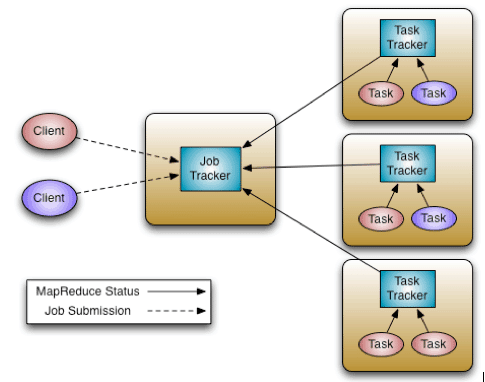
\includegraphics[height=70mm]{yarn-architecture}
\caption{The actors in YARN.}\label{fig:yarn-architecture}
\end{figure}

As shown in the Figure ~\ref{fig:yarn-architecture}, we have these actors:
\begin{itemize}
  \item The ResourceManager (RM), that manages resources in the cluster among all the applications.
  \item The NodeManagers (NM), agents running on each node of the cluster, that monitor YARN Containers, local resources and report the same to the RM.
  \item The ApplicationMaster, a specific framework module, which interacts with the assigned nodes, through the NM, to execute and monitor the tasks in the YARN Containers.
\end{itemize}

Although there is this separation, Hadoop YARN is defined as a monolithic cluster scheduler anyway \cite{yarn_vs_mesos}. That is because the scheduler logic to assign resources, is implemented only in the ResourceManager: in other words, the application-specific framework has no control at all in this process. In the context of autoscaling could be an issue: sometimes it could be useful to exploit autoscaling to maximize the performances of a specific job. It is quite hard to make it happen because we do not have control over the scheduling algorithm. A solution could be creating an ephemeral cluster to run only a job: it is not so much complicated in a cloud environment after all.

Monitoring the YARN metrics is the key step for autoscaling: analyzing them we could understand the current status of the whole cluster and make scaling decision accordingly. At this point we are in front of two big challenges:
\begin{enumerate}
  \item Selecting the most significant set of metrics, that capture as much information as possible about the current cluster status.
  \item Implementing a policy that exploits the selected metrics in an effective way. Here it is really important to have a deep knowledge about how YARN works, in order to implement a mechanism which harmoniously runs with the scheduler running in the RM.
\end{enumerate}

Last but not least, YARN provides us with an important feature: graceful decommission \cite{graceful_decom} of the Node Managers. In a dynamic context, where we can smartly detect wastage of resources, it is really important to make the deletion of the nodes in a reliable and safe fashion, in order not to destroy running tasks. Otherwise, we force the running framework to reschedule failed tasks, making slower the job or, in unlucky cases, making it fail. Thanks to this feature, we can remove nodes waiting for the completion of running tasks, avoiding to schedule new ones on them.   

\subsubsection{YARN metrics}
This a quick list of the most relevant YARN metrics exposed by the Resource Manager:
\begin{itemize}
  \item \textit{AllocatedMB}, the amount of allocated memory
  \item \textit{AllocatedVCores}, the number of allocated virtual cores
  \item \textit{AllocatedContainers}, the number of containers deployed in the cluster
  \item \textit{AggregateContainersAllocated}, the cumulative number of containers deployed in the cluster
  \item \textit{AggregateContainersReleased}, the cumulative number of released containers
  \item \textit{AvailableMB}, the amount of free memory
  \item \textit{AvailableVCores}, the number of free virtual cores
  \item \textit{PendingMB}, the amount of requested memory to be fulfilled
  \item \textit{PendingVCores}, the number of virtual cores to be fulfilled
  \item \textit{PendingContainers}, the number of containers to be fulfilled
  \item \textit{NumActiveNMs}, the number of active NodeManagers
  \item \textit{NumDecommissionedNMs}, the number of decomissioned NodeManagers
\end{itemize}

\section{Apache Spark}
After storage and resource management, data processing is the last of the three main aspects that we should consider when talking about Big Data. Nowadays Apache Spark \cite{spark} is absolutely the most popular framework, thanks to its great performances, ease to use and flexibility both for supported platforms (YARN, Mesos, Kubernetes) and use cases (such as SQL, Streaming and Machine Learning tasks).
\begin{figure}
\centering
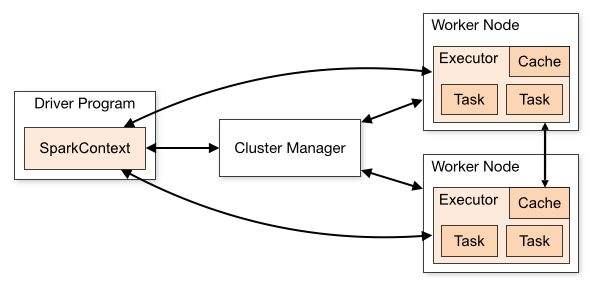
\includegraphics[height=70mm]{spark-architecture}
\caption{The Spark components.}\label{fig:spark-architecture}
\end{figure}
Spark uses a master/worker architecture. In its domain, as shown in Figure ~\ref{fig:spark-architecture}, we can find two types of actors:
\begin{itemize}
  \item The SparkDriver, the master, that negotiate with the cluster manager (i.e. YARN) for resources where to execute tasks.  
  \item The Executor, the process worker on each assigned node, that runs the tasks in the spawned threads.
\end{itemize}
One of the most important Spark features, that actually allows having great performances, is the so-called Resilient Distributed Dataset (RDD): it is the abstraction of the data the frameworks is dealing with. The RDD is split in small partitions, each of those maintained in the main memory of the Executors and processed in parallel by different tasks. In this way, all the write/read operation from the secondary memory, which is the case of Hadoop MapReduce, are avoided and we do not introduce significant overhead which slows down the entire workflow and could have a huge impact especially in iterative algorithms.

The theory behind Spark is quite vast, but we are going to review the fundamental concepts to have a general idea about how it works and to properly understand the following section "Dynamic Resource Allocation".

\subsection{Scheduling of stages and tasks}
The operations that we can use for a Spark job script are classified into two categories:
\begin{itemize}
  \item Transformation, where the input and the output is an RDD  
  \item Action, where the input is an RDD and the output is actually data in a file or variable
\end{itemize}
The first important concept is that all the Transformations are lazily evaluated. It means that each processing operation parsed in the code is not immediately evaluated. The DAG scheduler starts to build the Directed Acyclic Graph, where the node is a Transformation and the edge the relationship between the two ones. This approach allows having a global view of the entire workflow to apply many optimizations, such as reorganizing the order of the operations (in a way that the final result is not affected, of course) to minimize the size of intermediate data and speed-up the process.
The relationship between two Transformations could be of two types: Narrow or Wide. The first one means that each partition of the parent RDD is used by at most one partition of the child RDD; in few words, the single thread applies the transformation in its chunk of RDD. The second one means that multiple child partitions may depend on one partition of the parent RDD; this is the case when a Shuffling is needed, for example when we have to perform operations grouping by some keys. For this reason, in the DAG we can notice the so-called Stages: Wide transformation results in stage boundaries. The DAG scheduler is actually Stage-oriented because it works on the relationships between transformations and, as consequence of this, stages.
At this point of our journey, we can focus our attention what is inside a single stage: there are many tasks, that will be executed in the threads spawned by the Executor. Connecting the dots, a Spark will request the RM for YARN containers, because each Executor will run within them. The close relationship between YARN Container and Spark Executor is really important for the next step when we will introduce a key feature implemented in Spark, really useful for autoscaling.

\subsection{Dynamic Resource Allocation} \label{spark_dra}
Spark provides a mechanism \cite{spark_dra} to dynamically adjust the resources the application occupies based on the workload. This means that the application may give resources back to the cluster if they are no longer used and request them again later when there is demand. Specifically, the Spark engine continuously monitors the pending tasks queue and, when it realizes that the entire process is going to slow down too much, it triggers a request to the RM to allocate new Executors that, in turn, will create new threads to consume the pending tasks. On the contrary, when it realizes that there are no pending tasks and only a portion of the allocated Executors are actually used, it will release those idling.
The policy to request RM for new resources is inspired by the "TCP slow start" mechanism: at each time interval the monitoring check is performed and, if there is the need for new Executors, it will be requested only one, and then in each round increases exponentially from the previous round until the number is enough to consume all the pending tasks. Thanks to this approach, an application should request executors cautiously in the beginning in case it turns out that only a few additional executors is sufficient; but at the same time, it should be able to ramp up its resource usage in a timely manner in case it turns out that many executors are actually needed.
It is clear that this job-oriented mechanism is complementary to our cluster-oriented autoscaler: our mechanism should indulge its requests, placing new nodes into the cluster to accommodate more Executors, and then remove them when they are no longer useful.

\section{Google Cloud Platform}
The availability of high-capacity networks, low-cost computers and storage devices as well as the widespread adoption of hardware virtualization, service-oriented architecture, and autonomic and utility computing has led to growth in cloud computing \cite{cloud}. Thanks to cloud computing, companies no longer need to care about their on-premise infrastructures, spending both economic and human resources for operations on those. In the world where "everything as a service" is the way, people working at the companies can focus better on their job and work only on what matters for their business.
Among the most important cloud services providers, such as AWS \cite{aws} and Azure \cite{azure}, we can find Google Cloud \cite{gcloud}. They provide must-have services in the categories of computation, storage, databases and data warehousing, big data, machine learning and so on. In our context we can briefly mention those that we are going to actually use:
\begin{itemize}
  \item Compute Engine \cite{gce}, to deploy different kind of Virtual Machine where the software is going to run.
  \item Storage \cite{gcs}, to save important data and scripts.
  \item Kubernetes Engine \cite{kube}\cite{gke}, which expose the Kubernetes cluster where to deploy our containerized application.
  \item Dataproc \cite{dataproc}, to easily create ephemeral Hadoop clusters where to run Spark jobs.
\end{itemize}

Undoubtedly, Google Cloud Dataproc is the "first-class citizen" service, allowing us to create clusters but also dynamically reconfigure them based on autoscaling directives.

\subsection{Cloud Storage Connector}
An important problem we raised during the introduction to Hadoop is that we cannot rely on HDFS because of the not-indifferent overhead it introduces and in addition, it is possible that during autoscaling actions we will end up with a too small cluster to store all the data to be processed. It is necessary to store data in a different place and ship the chunks to Spark Executor only then they need. Apache Hadoop actually supports different file-systems: it is necessary to implement the class \textit{org.apache.hadoop.fs.FileSystem}, in order to expose the requested interface to perform the required semantics on files. Specifically, this is the list of operations that should be atomic:
\begin{itemize}
  \item Creating a file.
  \item Deleting a file.
  \item Renaming a file.
  \item Renaming a directory.
\end{itemize}
Of course in this way we are violating the "data locality" principle, a fundamental concept in the Big Data environment; in this case, we should rely on the performances offered by the internal network where our VMs run, inside the Google Cloud environment. Google Cloud Storage, as mentioned in the previous section, is our solution to store files to be processed. Using by the Cloud Storage Connector \cite{gcsconnector} we could easily access data stored in Storage from our Spark job, simply opening a file with \textit{"gs://<path-to-file>"}. Be aware that Cloud Storage is not a proper file-system, it is actually an object store. The interface offered by this kind of service corresponds to simply HTTP verbs rather than POSIX-like. In addition, they are design to be really high available so \textit{eventually consistent}. In few words we should be aware that they could fail in meeting the following features, guaranteed with HDFS:
\begin{itemize}
  \item Consistency, because of \textit{eventually consistent} design.
  \item Atomicity, because operations are not atomic.
  \item Durability, because it relies on the HTTP PUT operation that could fail.
  \item Authorization, because there is no conventional way to store metadata to handle owner, group and permissions.
\end{itemize}

\section{Elastic for YARN}
The validation and evaluation processes, in our scope, requires the visualization of the YARN metrics. Only in this way we can assess the behaviour of the mechanism, checking if it meets the requirement about resource savings and perfect utilization of the cluster. There are existing ready-to-use solutions out there: \textit{Google Stackdriver} \cite{stackdriver} and \textit{Ambari} \cite{ambari}. First, we will briefly discuss the advantages and drawbacks of these, then explain our solution based on \textit{Elastic Stack} \cite{elastic}.

\subsubsection{Google Stackdriver}
Pros:
\begin{itemize}
  \item No configuration required, it is perfectly integrated for each GCP service.
\end{itemize}
Cons:
\begin{itemize}
  \item Really expensive.
  \item Metrics not really precise with Google Dataproc.
  \item Flexibility: no customization and missing single-metric details.
\end{itemize}

\subsubsection{Apache Ambari}
Pros:
\begin{itemize}
  \item Designed for Apache Hadoop.
\end{itemize}
Cons:
\begin{itemize}
  \item Incompatibility with Google Dataproc.
  \item It requires Grafana \cite{grafana}, meaning additional configuration, for more flexibility.
\end{itemize}

\subsubsection{Our approach: Elastic Stack}
The solution based on the tools provided by the Elastic Stack is at the same time the simplest one and really effective. We can leverage the existing Elasticsearch cluster used in the company; in addition, Elastic provides tools like Kibana \cite{kibana} and Metricbeat \cite{metricbeat}, which allow us to collect metrics in a reliable way and ensure great flexibility about manipulation and visualization. There is no existing Metricbeat module for YARN but we can overcome the problem: it is available the module \textit{Jolokia} \cite{jolokia_mb}, useful to collect metrics from Jolokia agents \cite{jolokia} running on a target JMX server. Jolokia software is actually a JMX-HTTP bridge that allows you to access the metrics exposed in the Java Virtual Machine in an easier way. The only configuration task that we have to perform is to install and configure Metricbeat in the master node of each cluster and attach a Jolokia agent to YARN JVM: all these tasks could be easily executed automatically during the start-up of a new cluster, exploiting Google Initialization Actions \cite{dataproc_init_actions}.

\chapter{A piece in the puzzle: OBI}
The autoscaler that we are going to study is just a module inside a greater schema: OBI, Objectively Better Infrastracture. It is a software stack focus on cloud resources management. It aims to remove the entity "cluster" for the end-user who just wants to focus on their analytic applications. The software will take care of both of the ephemeral Spark clusters, transparently created through the Dataproc API, and of the incoming jobs, smartly deployed on them. To minimize time and cost expenditures, it implements many resource optimization mechanisms. It was designed and implemented by a team of three people, myself included, in parallel with my studies on the autoscaler. In the next chapter, we are going to see the architecture, the relationship between modules and the importance of the autoscaler.

\section{Architecture} \label{obi-architecture}
The two most important objectives are \textbf{run everywhere} and \textbf{lightweight}. Portability is one of the most important aspects: OBI should be as general as possible, in order to run on every environment with the minimum effort. To achieve this goal, the modules will be packed in Docker containers, allowing us to run the software also on Kubernetes (or other containers orchestrators). In addition, the implementation of logic and communication should be really simple but effective at the same time. It should run really fast in order to be really reactive on each change that happens on the managed clusters. Achieving this goal in the logic implementation of the modules is really challenging and an ongoing process. In order to make the communication really efficient but also reliable, we exploited gRPC \cite{grpc} library: it is the Google framework to implement Remote Procedure Call, based on Protocol Buffer \cite{protobuf} to exchange data, a really efficient and cross-platform serialization mechanism. Last but not least, the programming language: all the modules are implemented in Go, which allows us to write really efficient code with much less effort compared to C++/Java. The Figure ~\ref{fig:obi-architecture} shows the final architecture: 
\begin{figure}
\centering
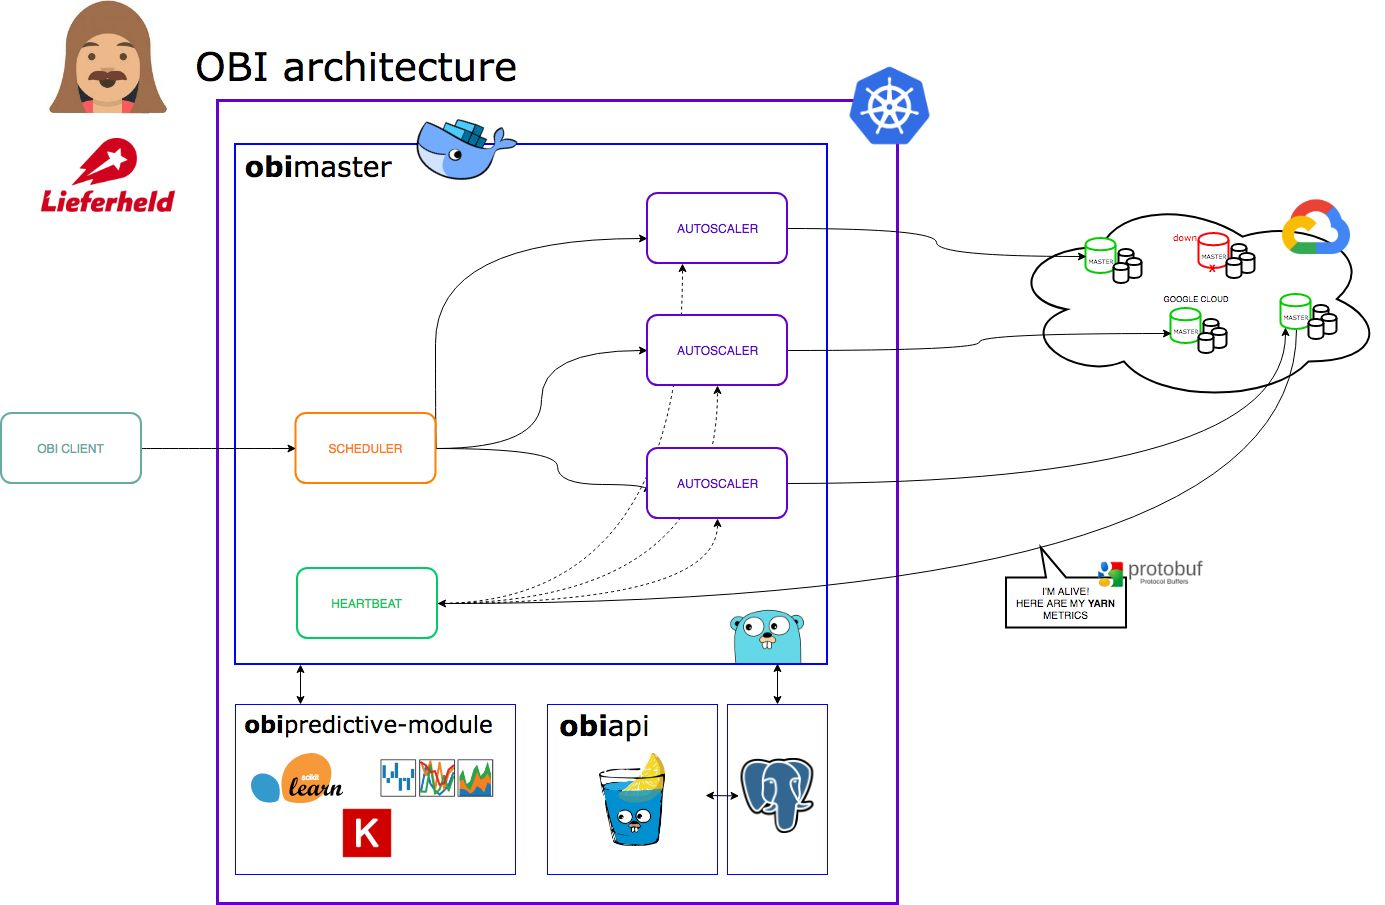
\includegraphics[height=70mm]{obi-architecture}
\caption{OBI architecture.}\label{fig:obi-architecture}
\end{figure}

\subsection{Heartbeat} 
The heartbeat module is crucial to get the current state of all our clusters. Remembering the lightweight principle, the operations of this module are extremely simple: in each master node of the clusters, a daemon script runs every \textit{t} seconds, sending all the metrics. The data is serialized using by Protocol Buffer to achieve high compression and sent on UDP packets in order not to introduce too much overhead. The receiver listens for these packets and, every time it receives the data from a specific cluster updates the sliding metrics window in a concurrency-safe fashion. If it does not receive anything from a cluster within a timeout interval, it will remove this last one from the pool.

\subsection{Scheduler}
In a cloud-based environment, we have to rethink our approach about job submission: we do not have long-living on-premise clusters. We work with the so-called "ephemeral model" \cite{ephemeral_model}: only when the user needs to submit jobs, he will create a specific cluster on the cloud, submit the jobs and delete it when every task has finished. In this way, we pay for what we actually use. 

The solution implemented by competitors, the "cluster pooling", is based on a different idea: keeping a pool of existing cluster and, upon job submission, select one of them. The weakness of this solution is that it is in contrast with the ephemeral model we have just talked about, and represents a wastage of money.  The only benefit we could have from this approach is cutting cluster initialization overhead. In the case of Google Dataproc we are talking about 1 minute, that is a negligible time saving considering that, in general, batch jobs have a "best-effort" priority, with no strict time constraints (such as in real-time application, front-end services and so on).

The main goal of the OBI scheduler is grouping together jobs submitted by different users in the same time period, in order to reduce the number of spawned cluster. The scheduler can accommodate many little jobs in a single cluster or one heavy and few light ones, for example. In this way, the module does not affect too much the performances of every single job. 

These are the main concepts of the OBI scheduler:
\begin{itemize}
  \item There are \textbf{N priority level}
  \item \textbf{For each} level, we have \textbf{many bins}
  \item \textbf{One bin} contains \textbf{many job}
  \item Upon job submission, the new size of the current bin is checked: if it exceeds the \textbf{threshold}, another empty bin is added in the level
  \item When the \textbf{level-timeout} expires, all \textbf{the jobs in a bin} will be deployed in \textbf{single cluster}
\end{itemize}
					
The scheduler is really flexible to allow the administrator to properly handle every kind of job in the platform, setting a longer timeout in order to maximize the packaging for low-priority jobs and vice versa. At the end of the day, he can configure:
\begin{itemize}
  \item The number of levels
  \item The value type of the bin (count or time duration)
  \item Threshold for bin size (60 minutes, 10 jobs, for example)
  \item Timeout for each level 
\end{itemize}

\subsection{Predictive module}
An important feature that allows the software to schedule jobs in a smarter way is the Predictive Module. Upon a job submission request is received by the master, before pushing the job into the scheduler logic, the time duration is estimated. The master sends all the relevant job and cluster details in order to attach in job instance the duration received in the answer.
Of course, this module is really environment-dependent and should be adapted to the typical jobs submitted. In general, the estimation is based on the most significant YARN metrics, such as memory and v-CPU information, but also and especially job information, like the number of processed files and their size. Despite its natural specificity, the implementation is modular, in order to allow external clients to train their own model based on any kind of Spark job, just implementing the interface with the software.

\subsection{API}
It is the module to expose relevant information for the users. Keeping in mind that the job is not immediately deployed into a cluster, with a delay-time dependent on the priority, it is really important to inform the users about the job status, log files and so on, in order that they could implement the logic for precedence constraints, failure handling and other related problems. The web server is implemented in Golang, specifically using the library GIN \cite{gin}. All the data are fetched from a PostgreSQL, as explained in the next section "Fault tolerance".

\section{Authentication and authorization}
All the communications between the client and the master are implemented using by Remote Procedure Calls. It is necessary to make these communications secure and only with authorized users. Many authentication mechanisms are built-in to gRPC: in the case of OBI, we exploited the SSL/TLS mechanism, in order to authenticate the server and encrypt all the messages exchanged. In addition, we use NGINX as SSL Termination and Reverse Proxy, in order to simplify the backend services. The unencrypted packet is then sent to the OBI master: in the header, gRPC allows to specify the user credentials, and a middleware checks if an account with that username and password exists in the database. 

\section{Fault tolerance}
Every software system has to care about failures, both software and hardware ones. The main goal is ensuring the entire system is not stopped, but it is capable to continue its operations introducing as little as possible service outage client-side and avoiding a total breakdown.
Two big steps towards an effective fault tolerance system are \textit{microservices architecture} and \textit{deploying on Kubernetes}.
The first one, among the many advantages, improves fault isolation: in a monolithic architecture the failure in a specific component leads to the failure of the entire system; on the contrary, with an architecture where we have many running services loosely coupled, we can improve fault isolation. It is important to remark the word \textit{improve} because we should keep in mind that all the components communicate each other: a severe failure in one or more service could have a not-indifferent impact on the whole system.
Kubernetes is today one of the best platforms where to run microservices systems. It offers many solutions in order to make them scalable and reliable. One of the most simple ones is ReplicaSet: in the case of stateless applications, such as the Predictive Module in our case, we can just create a Deployment that manages many replicas of the same software. In this way we can scale out the specific service and decrease the chance to have an outage for it, having more replicas ready to handle incoming requests. For the OBI master, we cannot follow this approach, because it maintains in-memory the state of the entire system. In addition, a failure in the master means that the entire system is not reachable by the end users: we have the so-called Single Point of Failure. In this case, the software relies on the Restart Policy:  Kubernetes detects the failure of the OBI Master and will care to restart the component again. At this point, we need a persistent layer, in order to trigger a recovery mechanism and recreate the state of the Master just before the failure.
At each action that modifies the current state of the OBI-Master, the new state is persisted to a PostgreSQL database.
The last point in order to tackle failures completely is the fault-tolerance for the database itself. The system relies on Stolon \cite{stolon}, an existing platform to ensure High-Availability for PostgreSQL. Of course, it leverages Kubernetes to achieve this: it uses not only the already mentioned features but also the so-called StatefulSet \cite{kube_statefulset}. It is the most important Kubernetes Object to manage stateful applications, that is the case. Stolon maintains many running PostgreSQL instances, each one in a Pod with a unique identifier, and just only one is the leader, i.e. the replica in charge to satisfy the write operations. The standby instances could satisfy only-read operations, because,  its state is synchronized with the master. In addition, to persist the application state on disk, each instance is bounded to a Persistent Volume, a storage-like resource that is bounded to the pod unique identifier \textbf{but} has a lifecycle independent of the individual pod that uses it. Last but not least, Stolon implements the logic to elect a new master when the old one is declared failed, in order to have nearly-zero downtime service.

\subsection{Deployment example on Kubernetes}
As discussed in the architecture section, the software is able to run on every environment with the minimum effort, thanks to containerization. However, we prefer Kubernetes for all the reasons discussed so far. In this environment we can apply the microservices architecture discussed so far, with the following components and respective Kubernetes Objects:
\begin{itemize}
  \item Master
  \begin{itemize}
  	\item Deployment to manage the Pod with replication factor equal to 1
  	\item NodePort service to expose an endpoint for receiving heartbeats from clusters.
  	\item LoadBalancer service to expose a public endpoint for accepting new job requests from the client.
  	\item Ingress NGINX-based to accept secure gRPC communications.
  	\item ConfigMap to load the yaml-like configuration file.
  	\item Secret to store the JSON file containing the Google Cloud credentials.
  \end{itemize}
  \item Predictive module
  \begin{itemize}
     \item Deployment to manage the Pod with replication factor equal to 2.
     \item ClusterIP service to expose it to the master.
  \end{itemize}
  \item API
  \begin{itemize}
     \item Deployment to manage the Pod with replication factor equal to 2.
     \item LoadBalancer service to expose a public endpoint for accepting requests.
     \item Ingress NGINX-based to accept only HTTPS requests.
  \end{itemize}
  \item HA-PostgreSQL
  \begin{itemize}
     \item Deployment to manage the Pods running the Proxies with replication factor equal to 3.
     \item Deployment to manage the Pods running the Sentinels with replication factor equal to 3.
     \item StatefulSet to manage the Pods running the Keepers with replication factor equal to 3.
     \item ClusterIP service to expose the Keepers inside the cluster.
     \item ClusterIP service to expose the Proxies inside the cluster.
  \end{itemize}
\end{itemize}

It is really easy to reproduce the same environment on any Kubernetes cluster because everything is installed using by a Helm \cite{helm} chart.

\chapter{State of the art}
In this chapter, we are going to explore existing solutions to perform autoscaling. We are going to analyze not only mechanisms tailored for Google Dataproc but even existing solutions in another context as a source of inspiration. At the end of each section, we will discuss the advantages and disadvantages of the approach, highlighting the features we should take care of.

\section{Google Cloud Dataflow}
Dataflow \cite{dataflow} is another service by Google for transforming and enriching data in stream and batch mode. Therefore the goal is data processing for many use cases, like for Dataproc.

The engine actually powering Dataflow is Apache Beam \cite{beam}. The key concepts are: 
\begin{itemize}
  \item Pipeline, the instance which encapsulates the entire data processing flow
  \item PCollection, a distributed data set to manipulate
  \item PTransform, the data processing operations that we can apply on PCollections
 \end{itemize}

The details about Beam are out of the scope of this thesis, but an in-depth explanation could be found in the programming guide \cite{beam_docs}. 
Despite many similarities with Apache Spark, there are important differences:
 \begin{enumerate}
 	\item Beam unifies Batch and Streaming pipelines. Indeed the PCollection could be bounded, meaning data come from a fixed source like a file, or unbounded, meaning data come from a continuously updating source via a subscription or other mechanism. In Spark, the developer has to implement two different versions of the code to manage the different pipelines.
 	\item API, a higher level of abstraction. The provided methods allow the developer to focus more on processing flow rather than on implementation details which could affect performances.
 	\item Portability. The same code can run everywhere thanks to Runner. We write once and we can execute it on different environments (on-prem, cloud) choosing the proper runtime Runners (Spark, Flink and others).
 \end{enumerate}
 
The most important advantage of using it is the abstraction. This service removes complexity on the client-side, managing all the operational tasks (scaling, availability, security, etc) and allowing the client to focus only on programming. It was designed with autoscaling in mind. Autoscaling relies on several signals to make decisions. Most of these assess how busy and/or behind workers are, including CPU utilization, throughput and the amount of work remaining (or backlog). Workers are added as CPU utilization and backlog increase and are removed as these metrics come down.

\subsection{What we learned}
Cloud Dataflow is really convenient when we have to perform classic data processing workflows, for the reasons we have discussed so far. Of course, we pay these nice features with flexibility. When we need to perform more complex workflows (iterative processing, notebooks, Machine Learning) we cannot rely on the simplicity of Dataflow, we have forced to use the classic/popular architecture Hadoop/Spark. It would be convenient to create the same abstraction level in this last environment, and OBI represents a step in this direction, exposing a job-oriented interface rather than cluster-oriented. Of course, we need a mechanism to emulate the autoscaling feature offered in Dataflow. As discussed in the Paragraph \ref{spark_dra}, in Spark there is the Dynamic Resource Allocation mechanism in order to dynamically adjust the resources your application occupies based on the workload. The mechanism is really similar to the autoscaling mechanism implemented in Dataflow but there is a big disadvantage: it does not care about the cluster. Probably if a job requires an additional worker for a computationally-intensive state, we will need additional cluster nodes in order not to affect other jobs which rely on the same resources. In Cloud Dataflow, on the other hand, the client only cares about jobs; we can imagine GCP as an autoscaled cluster and this is simply for developers. So, to conclude, we could implement an autoscaler that lies on top of Dynamic Resource Allocation mechanism and leverages in a similar way the signals exploited by Dataflow.

\section{Shamash}
Shamash \cite{shamash} is an autoscaling service tailored for Google Dataproc, developed by DoIT International. 

\begin{figure}
\centering
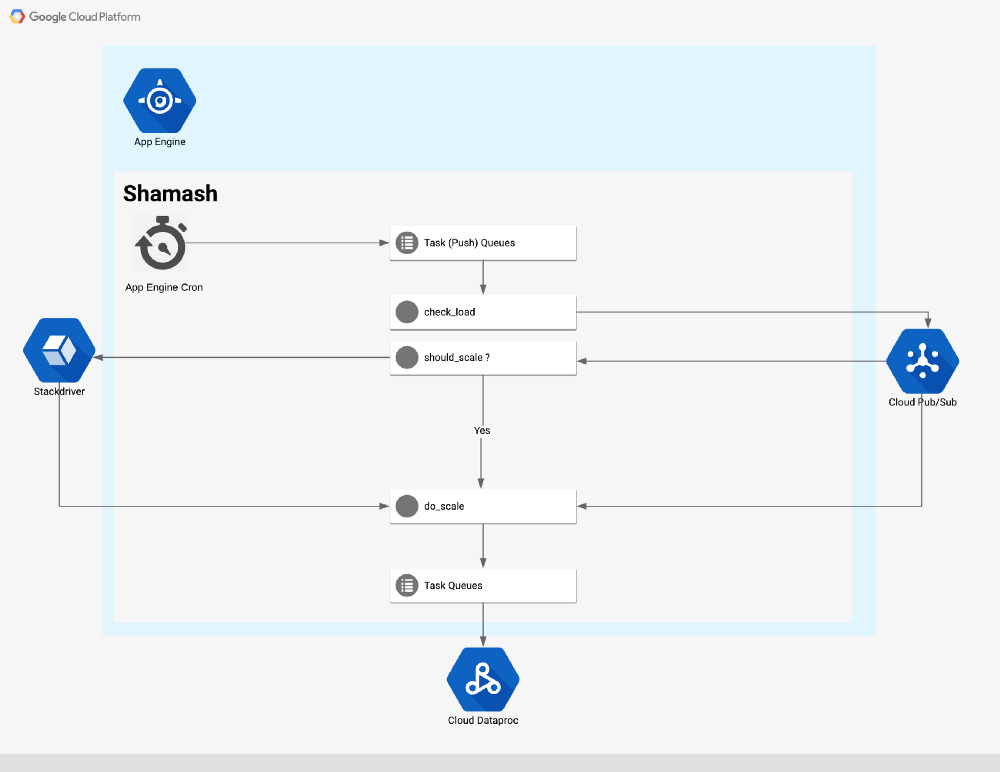
\includegraphics[height=80mm]{shamash}
\caption{The Shamash workflow.}\label{fig:shamash}
\end{figure}

In the Figure ~\ref{fig:shamash} the entire workflow is visualized. It is pretty straightforward:
\begin{enumerate}
	\item Every 5 minutes, in each managed cluster, a monitoring task is scheduled on the clusters machine.
	\item The monitoring task get the current YARN metrics and publishes them into a Pub/Sub topic.
	\item On a new Pub/Sub message, the function\textit{ check\_load} is triggered and retrieve the new message. If yes, another message will be published to another Pub/Sub topic.
	\item In the \textit{should\_scale} procedure the metrics are analyzed and the software makes a decision about the scaling action. 
	\item If a scaling action is required, the \textit{do\_scale} procedure will compute the number of nodes to add or remove.
\end{enumerate}

After Retrieving the information about the YARN Memory and YARN Containers, the following metrics are computed:
\begin{itemize}
	\item The YARN available memory percentage
	\item The YARN pending container percentage
\end{itemize}
At this point, it is possible to apply the scaling decision. The administrator could set four configuration threshold:
\begin{itemize}
	\item Up Memory Available percentage
	\item Down Memory Available percentage
	\item Up Pending Container percentage
	\item Down Pending Container percentage
\end{itemize}

The \textit{SCALE\_UP} action is triggered when:
\begin{enumerate}
	\item The current pending container percentage is greater than "up pending container percentage" threshold
	\item The current available memory percentage is less than "up available memory percentage" threshold
\end{enumerate}

On the contrary, the \textit{SCALE\_DOWN} action is triggered when:
\begin{enumerate}
	\item The current pending container percentage is less than "down pending container percentage" threshold
	\item The current available memory percentage is greater than "down available memory percentage" threshold
\end{enumerate}

In addition, there is the last option, that is \textit{SCALE\_TO\_MINIMUM}, when the current available memory percentage is 100%.
The last step to cover is determining the number of nodes to add or remove. There are two different strategies implemented: if there is enough historical data in Stackdriver, the new number of nodes is determined with a linear regression; on the contrary, the task is performed simply looking at how many containers fits in a single node and consequentially tune this number in order to have the minimum number of nodes that fit perfectly the current workload.

\subsection{What we learned}
The mechanism to get metrics introduces too much overhead due to the usage of Pub/Sub just to retrieve metrics: we can use directly StackDriver API to get this kind of information or custom efficient mechanism, as we did in OBI in the heartbeat module.
The choice to look at YARN Memory and Containers is quite good, they are the most important and discriminative metrics to get an idea about the actual utilization of the entire cluster. The scaling decision policy is too simplistic: it is true that "threshold-based" autoscalers are quite simple and effective, but in this case, it seems too much naive. In addition the developers do not provide any information about how they trained the regression model to determine the new number of nodes: I think that this solution is poorly generic, because it will learn the pattern from current jobs, that could differ in the workload slope. Last but not least, the idea of preemptible VMs is really good: for small jobs in duration, we can use them during scaling, in order to maximize the money saving. It is really important to remember that they could be killed at any moment, leading to tasks failures. For this reason it is not recommended for really long jobs: if too many failures occur, Spark will mark the job as failed, and of course we should run again the entire job.

\section{Spydra}
Spydra \cite{spydra} is a Google Dataproc wrapper, hiding the complexity of cluster lifecycle management, configuration and troubleshooting behind. It is really similar to OBI, actually being the software where we take inspiration from. It was developed at Spotify, as part of their effort to adopt the GCP platform for the data infrastructure.

Of course, one of the most important module in the Spydra context is the autoscaler module. The first important architectural choice to highlight is where the scaling algorithm runs: it is triggered every \textit{n} seconds on the master node of each cluster. This is a completely different approach we have seen so far: this solution allows to cut off every overhead related to metrics shipment. In addition, despite what we have seen in Shamash, the logic here is not 2-step-based (check if a scaling operation is needed and compute how many nodes), but it directly computes the new size of the cluster, making the module even more efficient. It is an important aspect not to neglect because the autoscaler should be really fast and reactive following the workload signal.

The metrics used are always the same, regarding YARN memory and YARN containers and in addition the number of active nodes. The new number of the nodes is determined around a configurable value: the factor. It is defined as the percentage of YARN containers that should be running at any point in time (from 0.0 to 1.0). At each time interval, based on the mentioned metrics, the current number of containers that the cluster can accommodate is computed, getting in this way the current factor. If this last indirect metric is less than the specified value, the autoscaler will scale up the cluster, and vice versa. The new number of nodes required is simply that size that allows satisfying the factor value. All the nodes added or deleted are preemptible VMs.

\subsection{What we learned}
The Spydra autoscaler does not introduce any remarkable characteristic with respect we have analyzed so far: it uses the same YARN metrics and the preemptible VMs. Its mechanism to get YARN metrics influenced the OBI heartbeat module, as discussed in Paragraph \ref{obi-architecture}. The autoscaler, every time is triggered, can read nearly real-time metrics, making decisions that are not "outdated". The configurable value "factor" is quite interesting, at least the idea it introduces: why do need to accommodate every pending container immediately? It is a good choice to tune this value on the job priority, for example: a low-priority job, because of a spike in its workload, could need a lot of containers; we can wait and satisfy the request only partially, hoping the spike will vanish after few seconds thanks to the job characteristics or the completion of other concurrent tasks. We can speculate, and if the resources demand is still high, it could be satisfied in more than one autoscaling action.

\section{Cloud Dataproc Cluster Autoscaler}
It is the autoscaler module, tailored for Google Dataproc, developed by Google \cite{google_autoscaler} and presented during the Google Cloud Next event in late July 2018. We cannot know all the implementations details, but the general algorithm, as explained in the documentation, is pretty clear and we can sum up in the following steps. 
\begin{enumerate}
	\item They introduce the concept of "cool down" period, during which the autoscaler collect all the metrics of cluster
	\item The number of nodes to add/remove, called "delta" in this context, is equal to Equation \ref{eq:delta_n}.
	\item If the delta is greater than the minimum fraction of workers, the scaling operation is performed. For example, if we have 20 nodes and this configurable value is 0.2, the scaling action is triggered if the delta is greater than 4.
\end{enumerate}

\begin{equation} \label{eq:delta_n}
\Delta N = \alpha\frac{\overline{P_{m} - A_{m}}}{W_{m}}  
\end{equation}
where:
\begin{conditions}
 P_{m}     &  YARN pending memory \\
 A_{m}    &  YARN available memory \\   
W_{m} &  worker YARN memory \\
 \alpha & scaling factor
\end{conditions}

\begin{figure}
\centering
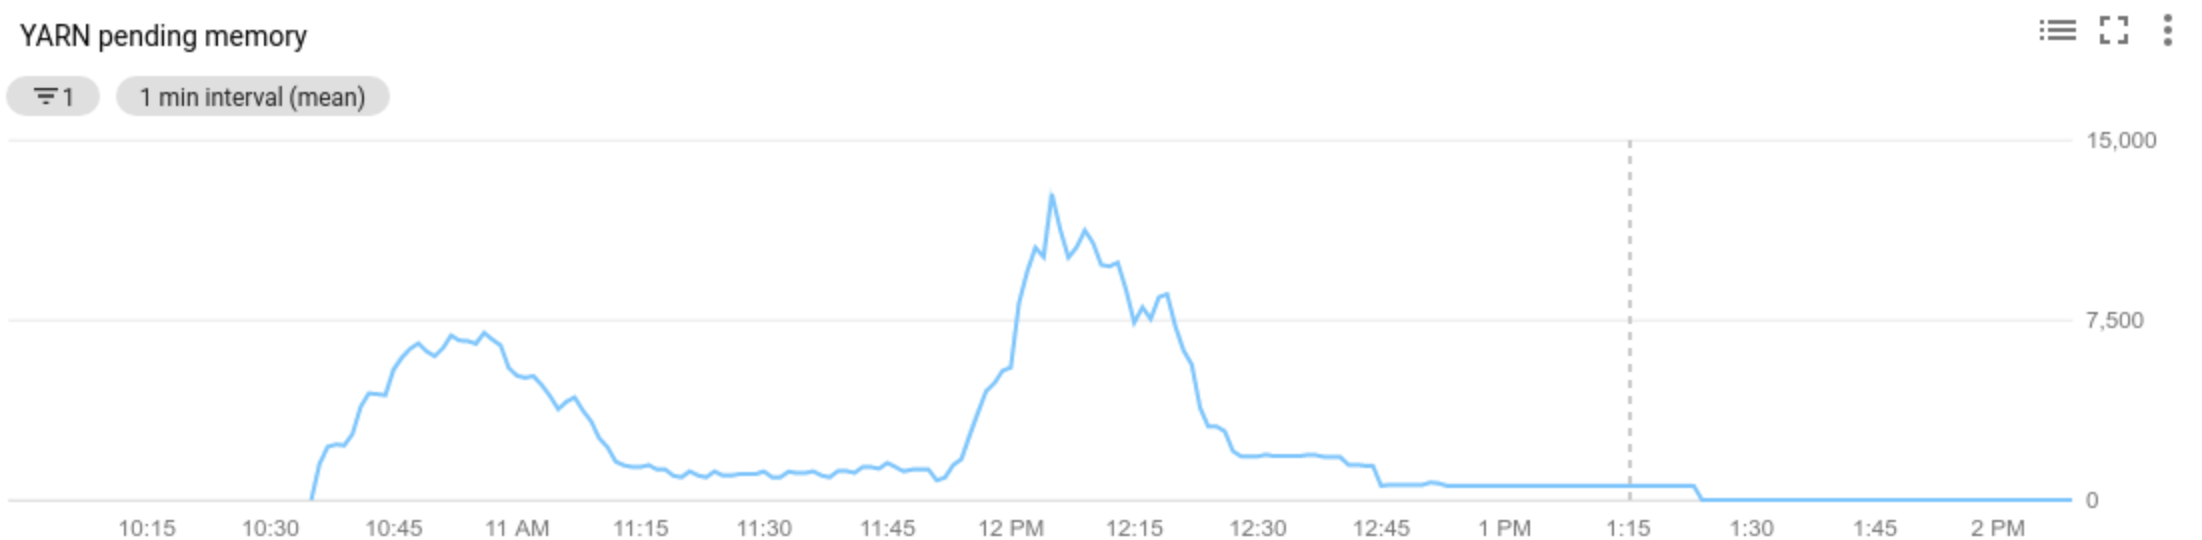
\includegraphics[height=40mm]{dataproc-example1}
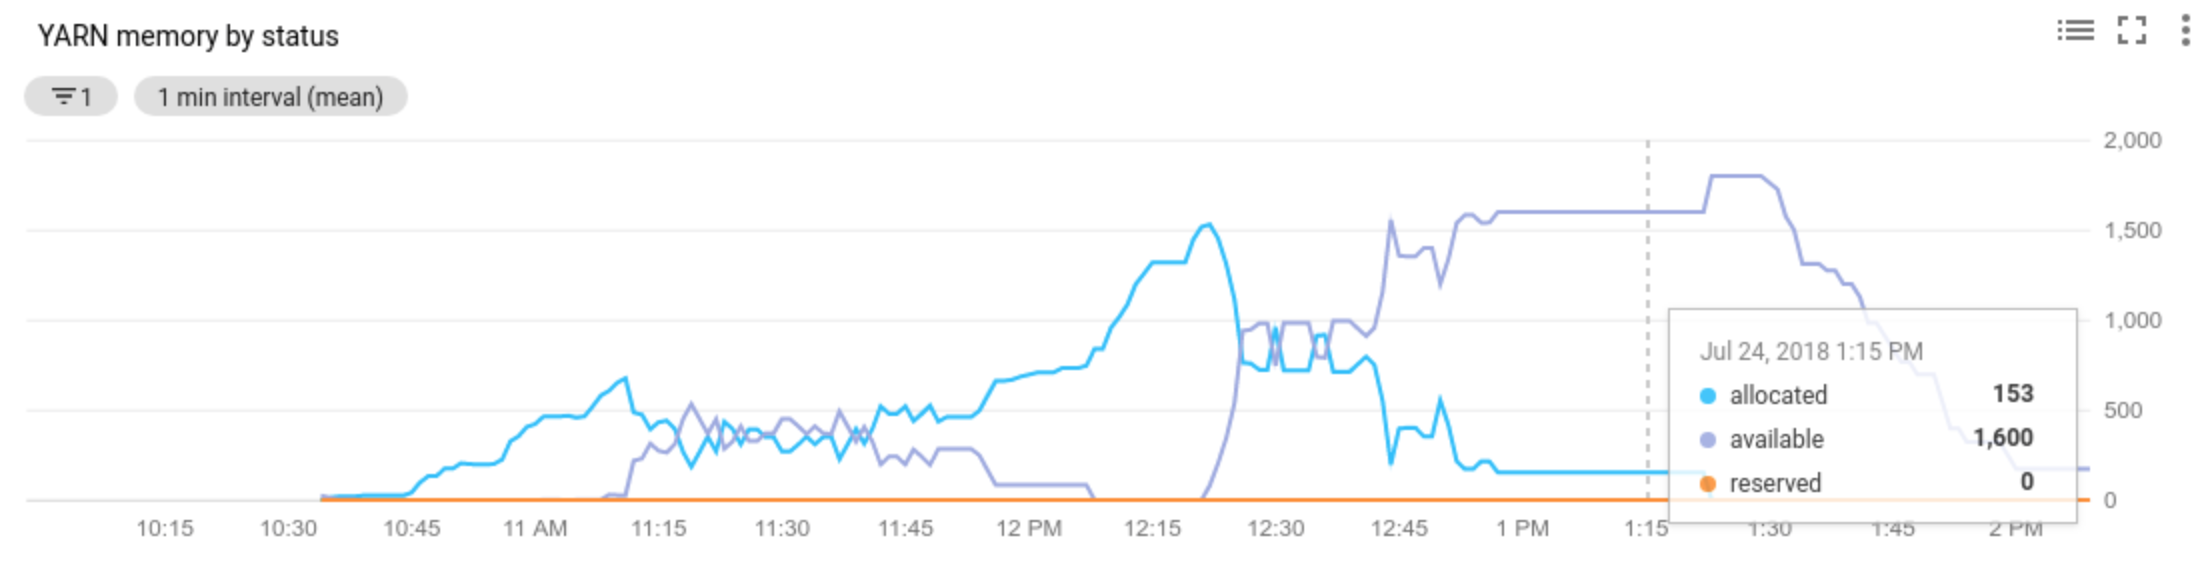
\includegraphics[height=40mm]{dataproc-example2}
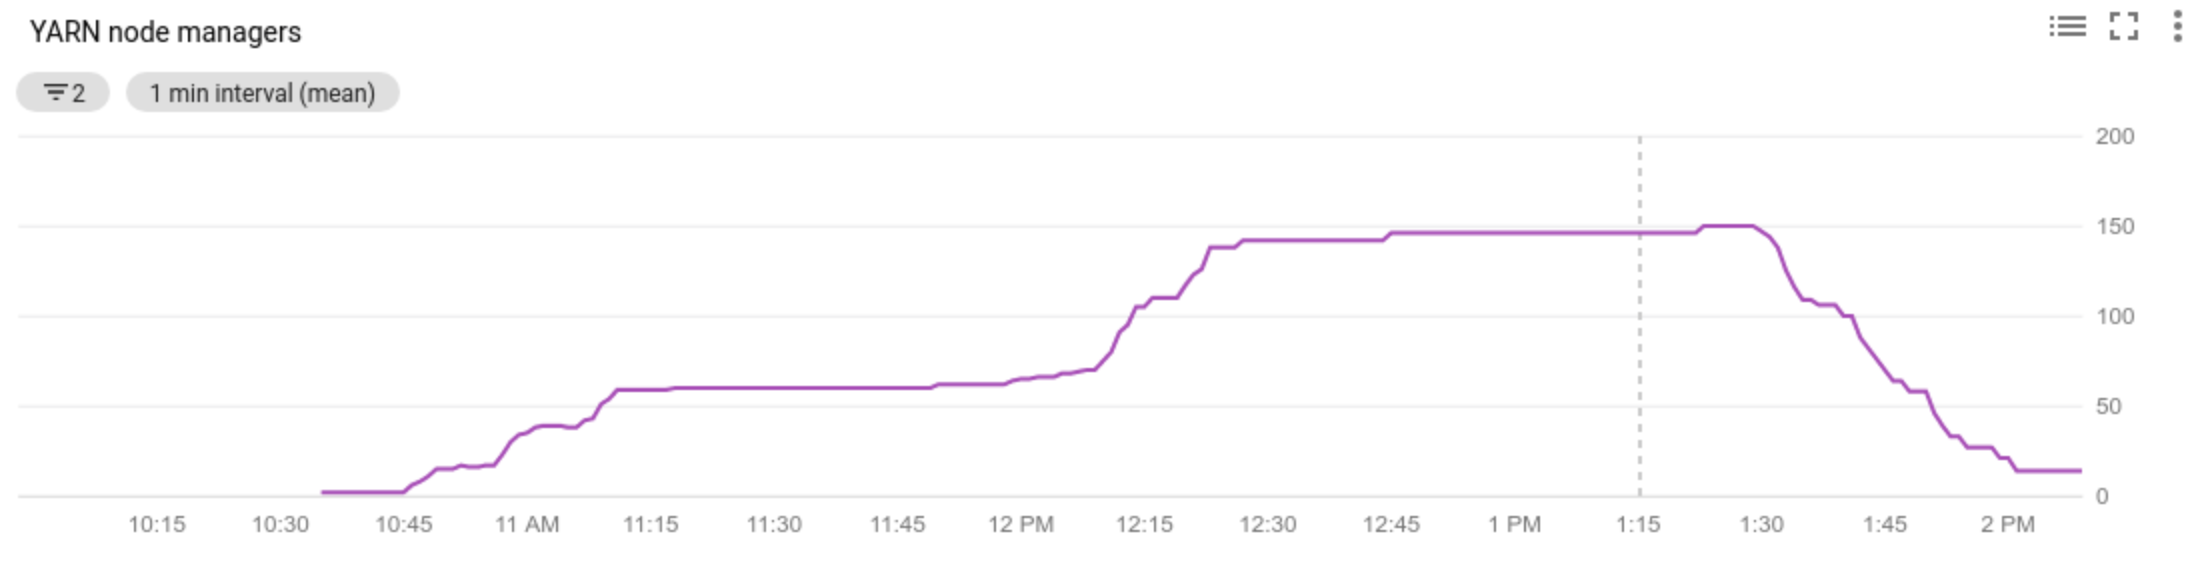
\includegraphics[height=40mm]{dataproc-example3}
\caption{Google Autoscaler in action.}\label{fig:dataproc-example}
\end{figure}

\subsection{What we learned}
The implementation provided by Google is really simple and general, in order to be effective in each environment with different jobs shapes. Engineers at Google leveraged on the same YARN metrics like the competitor tools, but they introduced a banal but really important feature not implemented in the other autoscaling mechanisms: the concept of windowing, the "cool down" period in this context. 
Making decisions based only on the really last metric could be completely misleading: the module should capture not only the current state of the cluster but even where it is going to be, trying to figure out the recent trends. In this specific case, the Google Autoscaler tries to evaluate, on average, how much memory it would have needed in order to have zero pending jobs during last period. The logic of "window analysis" it is the most important aspect which will heavily affect the autoscaler performances, and this is what we should focus on, mainly. One of the big drawbacks of Google implementation is the time window size: the minimum interval that could be set is 10 minutes, a huge interval that does not allow to promptly resize the cluster based on the real-time workflow.

\chapter{Design}
In this chapter, we are going to design the autoscaler. Specifically, we will discuss what we have inherited from the tools we have discussed about, the approach, the specific YARN metrics and finally the logic which drives the up/downscaling policies.

\section{The core points}
Based on what we have learned from the state of the art analysis, we can conclude:
\begin{enumerate}
	\item We absolutely need to get metrics about YARN Memory and Containers (at least).
	\item In order to maximize the saving, we can scale the cluster with preemptible VMs.
	\item The autoscaler could expose a tunable value as a scaling factor, to tune the chasing degree of the autoscaler based on jobs priorities.
	\item The autoscaler could ignore scaling actions that would add/remove a small number of nodes with respect the size of the whole cluster.
	\item The scaling decision should be based on the short-time window analysis, i.e. considering the last \textit{n} metrics just before the autoscaler was triggered.
\end{enumerate}

As discussed before, we have to focus on the logic that analyzes the window of metrics. All the autoscaler we have seen so far follow a threshold-based approach: it means the scaling action is triggered when a specific metric (either primary o secondary) is greater/less than a specified value in the configuration. There are other approaches out there, especially based on Machine Learning models and/or Time Series Analysis. The problem with these approaches is that they are quite rigid: in order to have good performances, it is necessary to have training data from the environment, allowing the model to learn the patterns implicitly present in the characteristics of the jobs. Despite everything, there is no guarantee the model will work after the big effort to collect data and train the most suitable one. This is one of the most important reasons that convinces companies to go with a threshold-based approach for real production services: it is really simple and quite effective in each environment. The main drawback is that the logic could be too much na{\"i}ve, especially when this approach is applied directly on the raw metrics offered by YARN: it is the case of EMR autoscaling \cite{emr_autoscaling}. The autoscaler by Google tries to do a step further for this approach, changing a little bit the common steps: it does not simply compare the metrics against a threshold, but it tries to compute secondary metrics and based on a relationship between them, compute directly the number of nodes that could be useful to add/remove. In this way, we could have still a simple design but much smarter and effective. We are going to follow this path, trying to design a logic capable of making smarter decisions.

\section{The window logic for scaling up}
Once we have fixed the must-have features for the autoscaler, we should focus completely on the logic we have to apply in each time-window. At this point, we should take a step back and remember what is the most important goal in this context: understanding where the cluster is going to go, the future state of it. Technically speaking, we would design a \textit{proactive} autoscaler: it means it could anticipate the future demands for resources. On the contrary, all the autoscaler we have seen so far could be defined as \textit{reactive}, meaning that the autoscaler reacts only when a workload issue occurred (probably too late!). This task is quite difficult without statistical models but we have already decided not to follow this approach, in order to apply the platform independence principle. A good trade-off could be an autoscaler in the middle between these two classes: neither purely proactive, because it is impossible with heuristics approach, nor purely reactive, trying to exploiting the evidence of the metrics to get the future trend of the workload, considering that in some cases it is actually impossible.

Before diving into our logic, we should take a look at the example shown in the Figure ~\ref{fig:flow-example-google}: it represents a possible case when the Google Autoscaler misses what we have discussed so far. It simply relies on the average of the unaccepted memory requests. In this case, a high memory request at the beginning of the window influences too much the final scaling decision. The negative average suggests the autoscaler to add nodes to bridge the missing memory gap, but from our rational point of view, we can easily understand that it is a totally wrong decision, as the colour gradient and the "future" part confirm. The root problem here is that the autoscaler treats the metrics as isolated single points in the time and, as a consequence, it cannot get any important information about their evolution.
  
\begin{figure}
\centering
\includegraphics[height=30mm]{flow-example-google}
\caption{The unfavourable case for Google Autoscaler. In each box the metrics about YARN Pending Memory and YARN Available Memory. The negative average is in contrast with the actual trend, highlighted by the color gradient.}\label{fig:flow-example-google}
\end{figure}

With a motorist metaphor, we can say that we are interested in average acceleration, rather than average speed. We should analyze each metric with respect to the previous one to get the trend of the workload. We can conclude this part by saying that we actually need two different kinds of rates:
\begin{itemize}
	\item The \textbf{pending rate}, to evaluate the trend for pending containers.
	\item The \textbf{throughput}, to evaluate the trend for containers decommission.
\end{itemize}

If the pending rate is greater than the throughput, the cluster cannot find enough resources to allocate new containers because it does not release the existing one, so it needs more nodes. In the opposite case, the cluster probably is over-provisioned because it continuously releases resources. Computing the difference between these two rates, we actually get the rate of containers that the cluster could not allocate immediately. Finally, we can now formulate the new delta returned by the autoscaling logic, as in Equation \ref{eq:delta_my}.

\begin{equation} \label{eq:delta_my}
\Delta N = \alpha(T - G)
\end{equation}
where:
\begin{conditions}
 T     &  Throughput \\
G    &  Pending growth rate \\   
 \alpha & scaling factor
\end{conditions}

This first formulation is really high-level but it is just to give the overall idea of the algorithm. In the next section, we are going to deep into this formula, adding more details and introducing the YARN metrics that allow us to estimate these two high-level rates. 

\section{Selection of YARN metrics}
In the previous chapter, we have seen that all the competitors' tools leverage on memory and container YARN metrics. Of course, these ones are really important and we are going to use them, but we should introduce some other information to evaluate if the cluster perfectly fits the workload or not. We need a metric to understand if the currently allocated resources are totally used all the time and, in case of pending containers at the same moment, we scale up the cluster. It is one of the biggest differences with respect the competitors: we could have pending containers but, if at the same moment the autoscaler notices that the resources are going to be released, we do not need to add new nodes. 
Among the YARN metrics mentioned in the introduction, the \textit{AggregateContainersReleased} might help us. In order to explain better its importance, we are going to analyze its behaviour during an expensive Spark job: the K-means, with the following set-up:
\begin{itemize}
	\item 300000 random sample.
	\item 40 centroids.
	\item 25 iterations.
\end{itemize}
The cluster configuration is the following:
\begin{itemize}
	\item 1 master node with 4 CPU and 15.0 GB of memory.
	\item 2 slave node with 4 CPU and 15.0 GB of memory.
\end{itemize}
The Figure \ref{fig:released-metrics} shows the result: there are 5 allocated containers (1 is for the Application Master e 4 containers to execute tasks). We can conclude that the YARN Resource Manager actually gave all the available resources to the job because only 2 containers fit in every node at maximum. We can notice these four containers are \textbf{never} released because of the high workload of the iterative algorithm. There are pending containers (not showed in the figure) for sure, in order to immediately execute tasks that could not find free space into the existing ones. But what YARN actually does is waiting for tasks completion and, instead of satisfying pending containers requests, schedule the pending tasks in the already allocated containers. At the end of the job, we can see they all are released at the same time because there are no longer tasks to schedule.

\begin{figure}
\centering
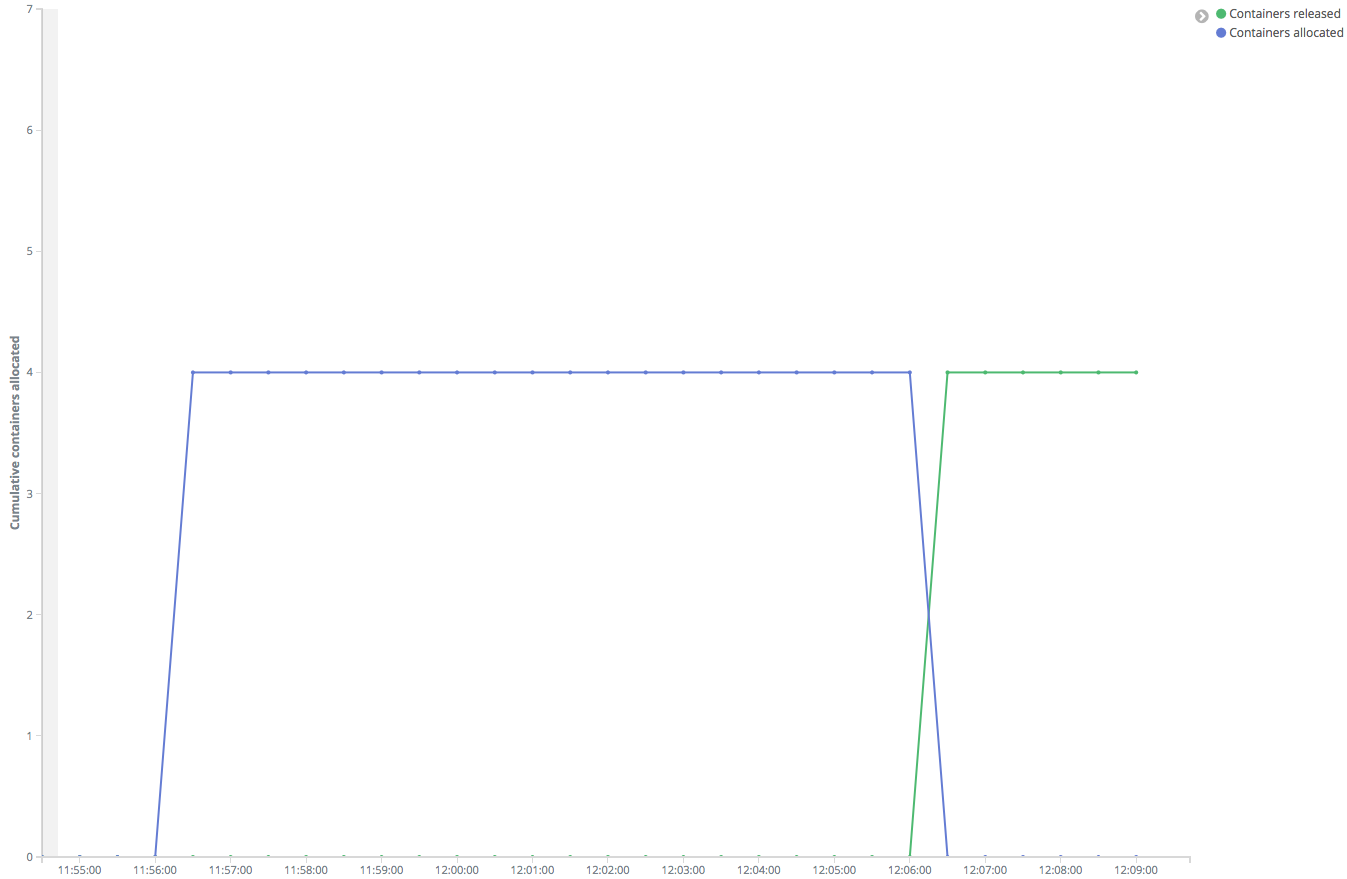
\includegraphics[height=80mm]{released-metrics}
\caption{The evolution of \textit{AggregateContainersReleased} and \textit{ContainersAllocated} during the execution of a K-means job.}\label{fig:released-metrics}
\end{figure}

At this point it is clear that we could use this metric we have introduced to compute the \textit{throughput} rate, as shown in Equation \ref{eq:throughput_my}. We have just obtained the first mentioned rate so far, to evaluate the trend for containers decommission.

\begin{equation} \label{eq:throughput_my}
T = \frac{1}{N_{w} }\sum_{t = 1}^{N_{w} }C_{r}(t)-C_{r}(t-1)
\end{equation}
where:
\begin{conditions}
 T     &  Throughput \\
C_{r}    &  The total number of released containers \\ 
N_{w}   &   The number of metrics points in the time window 
\end{conditions}

At this point, we need to compute the second rate, the \textit{pending growth} one. This case is quite simple because we just have to look at the \textit{pending-type} metrics like the competitors do. But even in this case, we could introduce a small detail to improve the actual estimation of the new resources needed. It could happen usually that both \textit{PendingMemory} and \textit{AvailableMemory} are greater than zero. It happens because YARN is going to use the free resources to satisfy the requests (at least partially) but this on-going process is not revealed by the metrics, updated only when the allocation process has done. For this reason, we could a find a third term in the Equation \ref{eq:growth_my}, where we compute the number of containers that will be allocated soon, simply dividing the total available memory by that one used to allocate a single container.

\begin{equation} \label{eq:growth_my}
G = max(0,\frac{1}{N_{w} }\sum_{t = 1}^{N_{w} }C_{p}(t)-C_{p}(t-1)-\frac{M_{a}(t)}{M_{c}})
\end{equation}
where:
\begin{conditions}
 G     &  Pending growth rate \\
C_{p}    &  The total number of pending containers \\  
N_{w}    &   The number of metrics points in the time window  \\
M_{a} & The available memory \\
M_{c}  & The memory allocated for a container
\end{conditions}

In this section we have deepened every term in \ref{eq:delta_my}, and now we could rewrite it in details as in Equation \ref{eq:delta_my_extended}.
\begin{equation} \label{eq:delta_my_extended}
\Delta N = \alpha(\frac{1}{N_{w} }\sum_{t = 1}^{N_{w} }C_{r}(t)-C_{r}(t-1) - max(0,\frac{1}{N_{w} }\sum_{t = 1}^{N_{w} }C_{p}(t)-C_{p}(t-1)-\frac{M_{a}(t)}{M_{c}}))
\end{equation}

\section{Downscaling}
Even if it could seem a simple operation, just the opposite of scaling-up, downscaling is completely another story. For this reason we should rethink the approach discussed so far. We have designed an algorithm in order to assess how many more nodes the cluster needs to fit perfectly the workload. All the sophisticated features we have described are going to fail because here we have a totally different goal. Right now the main objective was adding the minimum number of nodes as possible to meet the future demands of resources. In this case, the objective is even simple: remove unused nodes. And for a simple goal, we possibly need a simple design. In addition, a decoupled mechanism between scaling-up and scaling-down could be useful to tune differently the autoscaler in these two different cases. For example, the autoscaler could be "prudent" at adding nodes but really "aggressive" at removing them, at the same time. This is a feature that competitors completely ignored.
The simplest and most effective solution could be installing a daemon inside each node of the clusters, in order to query NodeManager's metrics and evaluate the activity level over a fixed time window. This mechanism is actually implemented in the autoscaling module of other platforms, such as Kubernetes. Unfortunately, we cannot adopt this solution because of Google API limitations: this mechanism requires the possibility to shut down a specific node. In "clouds terms", we need to call an API that allows us to shut down a specific VM where the NodeManager is running. The Dataproc API actually does not expose this functionality but it permits just to change the size. For this reason, the adopted solution is slightly different: if and only if the pending rate is equal to 0 (it means that the cluster is either perfectly sized or over-provisioned), the autoscaler computes the new size following a "compaction" approach. From the currently allocated memory information, it determines how many nodes fit in a single node of the cluster. the minimum number of nodes that allow having the same quantity of memory. Of course it is just an approximation: the memory allocation is spread out in the cluster: for example, assuming that a node could host 2 containers at maximum, we could have a situation where there are 2 nodes with only a container allocated each. The Equation \ref{eq:downscaling_my} formalizes what explained so far:

\begin{equation} \label{eq:downscaling_my}
\Delta N = N-\frac{C_{a}}{C_{n}}
\end{equation}
where:
\begin{conditions}
C_{a}    &  The total number of allocated containers \\  
C_{n}    &   The number of containers that fits in a single node \\
N & The current size of the cluster
\end{conditions}

\chapter{Implementation}
In this chapter, we are going to see the implementation in details. As anticipated in the Paragraph \ref{obi-architecture}, the programming language is Golang. It allows us to write efficient, multi-threaded code with the minimum effort compared to C/C++. As the first step in the part, we will introduce some of the basic concepts we need to know before diving in the code. Then we will analyze the most important chunk of the code and how we have implemented the semantics discussed in the previous chapter.

\definecolor{light-gray}{gray}{0.95}
\definecolor{commentgreen}{RGB}{2,112,10}
\lstset{ % add your own preferences
    frame=single,
    basicstyle=\footnotesize\ttfamily,
    breaklines=true,
    framextopmargin=50pt,
    commentstyle=\color{commentgreen},
    frame=bottomline,
    keywordstyle=\color{orange},
    numbers=left,
    numbersep=5pt,
    showstringspaces=false, 
    stringstyle=\color{blue},
    tabsize=4,
    backgroundcolor = \color{light-gray},
    language=Golang % this is it !
}

\section{Go in a nutshell}
Go is an imperative, statically typed programming language. The syntax is really similar to C with some modern characteristics (no parenthesis in the if statements, instant declaration/initialization). Like C/C++ we can work directly with pointers, but there is no support for pointer arithmetic. In addition, it compiles to native code to ensure great performances.  This is the classic \textit{"Hello World"} program:
\begin{lstlisting}
package main

import "fmt"

func main() {
    fmt.Println("Hello Go")
}
\end{lstlisting}

It is not a proper object-oriented language if we come from C++/Java. The first big difference is that we do not have classes: we can define structs, embedding properties, and we can define methods for them. We do not have the most important OOP concepts like inheritance, because creators tried to push for \textit{Composition over Inheritance}\cite{composition_inheritance}. In order to exploit polymorphism, Go offers \textbf{\textit{interfaces}}: they work as in C++ and Java, but there is no need for the programmer to explicit the interfaces that the struct is going to implement: just implementing all the defined methods, the interface is satisfied implicitly.
One of the key features is concurrency: Go was born when the multi-threading caught on, for this reason, it was designed with concurrency in mind. Launching a new thread, in this context \textbf{\textit{goroutine}}, to execute a specific function is really easy:
\begin{lstlisting}
// just a function (which can be later started as a goroutine)
func doStuff(s string) {
}

func main() {
    // using a named function in a goroutine
    go doStuff("foobar")

    // using an anonymous inner function in a goroutine
    go func (x int) {
        // function body goes here
    }(42)
}
\end{lstlisting}
Of course, there are many libraries to solve all the concurrency-related issues, especially about synchronization. They all are designed to be really easy to use: the idea is just to write only a few lines and everything will be managed behind the scene, the developer does not to worry about it. Explaining all these libraries is out of the scope of this chapter; we are going to introduce only \textbf{\textit{channels}}: they are typed conduit through which the different goroutines can send and receive values. In the following chunk of code, a comprehensive review of the channel usage:

\begin{lstlisting}
ch := make(chan int) // create a channel of type int
ch <- 42             // Send a value to the channel ch.
v := <-ch            // Receive a value from ch

// Non-buffered channels block. Read blocks when 
// no value is available, write blocks until there is a read.

// Create a buffered channel. Writing to a buffered channels 
// does not block if less than <buffer size> unread values have been written.
ch := make(chan int, 100)

close(ch) // closes the channel (only sender should close)

// read from channel and test if it has been closed
v, ok := <-ch

// if ok is false, channel has been closed

// Read from channel until it is closed
for i := range ch {
    fmt.Println(i)
}

// select blocks on multiple channel operations, 
// if one unblocks, the corresponding case is executed
func doStuff(channelOut, channelIn chan int) {
    select {
    case channelOut <- 42:
        fmt.Println("We could write to channelOut!")
    case x := <- channelIn:
        fmt.Println("We could read from channelIn")
    case <-time.After(time.Second * 1):
        fmt.Println("timeout")
    }
}
\end{lstlisting}

\section{The autoscaler package}
Inside the autoscaler package we could find two different parts:
\begin{itemize}
	\item The autoscaler module
	\item Policies
\end{itemize}

It is really important this separation because it introduces to modularity. The autoscaler is a general module in the OBI context with \textit{pluggable} policies. What we have discussed in the previous chapter it will be the autoscaling policy in this context. Now, with the following pieces of code, we are going to clarify the roles of these two complementary parts and what actually they do respectively.

In Go environment, the code is organized in the so-called packages; defining packages and declaring structs with methods inside, we can implement in a similar way we got used in an OOP language. In the \textit{autoscaler package}, first of all, we have defined the struct for the autoscaler module and the \textit{interface Policy} that must be implemented in order to build a pluggable policy. 
\begin{lstlisting}[caption={Autoscaler struct and Policy interface},label={lst:autoscaler}]
package autoscaler

import ...

// Autoscaler module resizes the managed cluster 
// according to the policy.
// The policy is a pluggable struct with a well-defined 
// interface to implement.
type Autoscaler struct {
	Policy Policy
	Timeout int16
	quit chan struct{}
	managedCluster model.Scalable
	allowDownscale bool
}

// Policy defines the primitive methods that must be 
// implemented for any type of autoscaling policy
type Policy interface {
	Apply(*utils.ConcurrentSlice) int32
}
\end{lstlisting}

In the code~\ref{lst:autoscaler} we can immediately analyze the properties inside the \textit{Autoscaler struct}:
\begin{enumerate}
	\item Policy, in the Policy struct that implements the interface and applied at each timeout.
	\item Timeout, is the time interval in seconds to trigger the policy logic.
	\item quit, is the channel to communicate with autoscaler goroutine, used for safely close the thread.
	\item managedCluster, the \textit{Scalable} cluster to scale periodically.
	\item allowDownscale, a setting to allow the downscaling or not.
\end{enumerate}

We can easily understand that this module controls the autoscaling behaviour from a higher point of view. In the architectural design of the code, we have an Autoscaler instance for each Cluster instance, and only the first one knows the second one. It is important to notice that from the autoscaler point of view, there is no specification about the cloud platform. It could be from Google Cloud, AWS, whatever: it must implement the \textit{Scalable} interface, it means that is a cluster that provides methods to resize itself during the execution. 
The boolean to block downscaling could be useful sometimes: the downscale operation, as we will discuss in the next chapters, is quite problematic for already running tasks. In the case where we are more interested in performances rather than cost saving, it could be exploited. 
After the initialization, where we specify the high-level information discussed so far, we can start and stop (see code~\ref{lst:ss-autoscaler}) the goroutine which applies the policy at every time interval.
The struct Policy, in order to be so, must implement the method \textit{Apply} that receives the window containing the last metrics and return an integer the could call \textit{delta}.

\begin{lstlisting}[caption={The start and stop methods for the autoscaler},label={lst:ss-autoscaler}]
// StartMonitoring starts the execution of the autoscaler
func (as *Autoscaler) StartMonitoring() {
	logrus.WithField("clusterName", as.managedCluster.(model.ClusterBaseInterface).GetName()).Info(
		"Starting autoscaler routine.")
	go autoscalerRoutine(as)
}

// StopMonitoring stops the execution of the autoscaler
func (as *Autoscaler) StopMonitoring() {
	close(as.quit)
}
\end{lstlisting}

The Start method essentially executes the goroutine called \textit{autoscalerRoutine}; the Stop one closes the \textit{quit} channel. If we take a look at code~\ref{lst:routine-autoscaler}, we can notice that before applying the policy, after timeout expiration, the routine tries to read from the channel: it will "read" the closing operation and the goroutine exits. In case of no closing operations on the channel, the plugged policy is executed getting the delta to update the cluster and then the goroutine goes to sleep for the timeout.

\begin{lstlisting}[caption={The autoscaler goroutine.},label={lst:routine-autoscaler}]
// goroutine which apply the scaling policy at each time interval
// It will be stop when an empty object is inserted in
// the `quit` channel
// @param as is the autoscaler
func autoscalerRoutine(as *Autoscaler) {
	var delta int32
	for {
		select {
		case <-as.quit:
			logrus.WithField(
				"clusterName", 
				as.managedCluster.(model.ClusterBaseInterface)
					.GetName()
				).Info("Closing autoscaler routine.")
			return
		default:
			delta = as.Policy.Apply(
				as.managedCluster.(model.ClusterBaseInterface)
					.GetMetricsWindow())

			if (delta < 0 && as.allowDownscale) || delta > 0 {
				as.managedCluster.Scale(delta)
			}
			time.Sleep(time.Duration(as.Timeout) * time.Second)
		}
	}
}
\end{lstlisting}

The last step to do is the implementation of the policy, all the semantics and design choices that we have already discussed during the previous chapter. The implementation (see code~\ref{lst:policy-autoscaler}) is actually really long. For this reason, we are going to break it into sections of lines and focusing completely on each one.

\begin{lstlisting}[caption={The implementation  of the autoscaling policy.},label={lst:policy-autoscaler}]
// Apply is the implementation of the Policy interface
func (p *WorkloadPolicy) Apply(
		metricsWindow *utils.ConcurrentSlice) int32 {
	var previousMetrics model.HeartbeatMessage
	var throughput float32
	var pendingGrowthRate float32
	var count int8

	for obj := range metricsWindow.Iter() {
		if obj.Value == nil {
			continue
		}

		hb := obj.Value.(model.HeartbeatMessage)

		if previousMetrics.ClusterName != "" {
			throughput += float32(hb.AggregateContainersReleased - 
				previousMetrics.AggregateContainersReleased)
			if hb.PendingContainers > 0 {
				memContainer := hb.PendingMB / hb.PendingContainers
				containersWillConsumed := hb.AvailableMB / memContainer
				pendingGrowth := float32(hb.PendingContainers - 
					containersWillConsumed - 
					previousMetrics.PendingContainers)
				if pendingGrowth > 0 {
					pendingGrowthRate += pendingGrowth
				}
			}

			count++
		}
		previousMetrics = hb
	}

	if count > 0 {
		throughput /= float32(count)
		pendingGrowthRate /= float32(count)

		workerMemory := (previousMetrics.AvailableMB + 
			previousMetrics.AllocatedMB)/previousMetrics.NumberOfNodes

		// compute the number of containers that fit in each node
		var containersPerNode int32
		if previousMetrics.AllocatedContainers > 0 {
			memContainer := previousMetrics.AllocatedMB 
				/ previousMetrics.AllocatedContainers
			containersPerNode = workerMemory / memContainer
		} else if previousMetrics.PendingContainers > 0 {
			memContainer := previousMetrics.PendingMB 
				/ previousMetrics.PendingContainers
			containersPerNode = workerMemory / memContainer
		} else {
			// unable to estimate the value - let's take the minimum
			containersPerNode = 2
		}

		if pendingGrowthRate == 0 && 
		previousMetrics.AllocatedContainers > 0 {
			nodesUsed := math.Ceil(
				float64(previousMetrics.AllocatedContainers 
					/ containersPerNode)
			)
			return int32(nodesUsed) - previousMetrics.NumberOfNodes
		}
		return int32((pendingGrowthRate - throughput) 
			* (1 / float32(containersPerNode)) * p.scale)

	}

	return 0
}
\end{lstlisting}

\subsubsection{Lines 9-37 | Rates computation}
In this section. we use the already mentioned metrics inside the window to compute the rates formulated in Equation \ref{eq:throughput_my} and \ref{eq:growth_my}. Of course, we start from the second one in order to compute, at each iteration, the difference with the previous one. In the end, we simply divide by the number of differences we summed just to compute the average. Keep in mind that, from the autoscaler point of view, we do not know the size of the window and in addition, it could not be completely full of metrics: in the first seconds of the cluster lifecycle, for example, we could have a window that contains only partially the metrics. The parameters that affect this aspect are the heartbeat time interval and the length of the metrics window, two factor that is not under the control of the autoscaler.

\subsubsection{Lines 39-55 | Computing other information about the cluster}
The additional information we need to apply the equations for scaling up/down are:
\begin{enumerate}
	\item The worker memory 
	\item The number of containers that fit in a single node.
\end{enumerate}
We cannot get these two parameters directly from YARN, for this reason, we need to compute them. The worker memory, i.e. the available memory for YARN context in the machine, is really simple to compute: just dividing the overall memory (the sum of available and allocated) in the cluster by the number of the nodes. This information is still useful to compute the second one we are interested in: the number of containers in a node is just the division between the worker memory and the memory allocated for a single container.
The container memory size could be computed simply looking at the ratio between the overall allocated memory in the cluster and the number of allocated containers. In order to have a resilient implementation, the code is a little bit complicated: we try to compute this information exploiting the "allocated-like" metrics; if it is not possible we exploit the "pending-like" ones otherwise we simply take the worst-case value.

\subsubsection{Lines 57-70 | Scaling up/down}
At this point, we have all the information we need. As discussed in the previous chapter we follow two different modelling approaches to distinguish the case of scaling up and down. If the pending rate is equal to 0 but we have allocated containers, the cluster could be over-provisioned: in this case, we scale to the minimum number of machines that we need to host the already allocated containers, assuming that each machine is with 100\% utilization. In the opposite case, we could need of a scaling up action: the function returns the delta defined in the Equation \ref{eq:delta_my_extended}.

\chapter{Results}
This chapter will be where we discuss the tests performed running real production jobs, deployed in clusters controlled by the implemented autoscaler We are going through different testing sets; specifically, we can tune the testing environment with the following factors:
\begin{enumerate}
	\item The types of jobs (computational intensive for long periods, with workload spikes and so on)
	\item The scaling factor of the autoscaler
	\item Downscaling enabled/disabled
	\item Timeout
	\item Gracefully Decommissioning Timeout
\end{enumerate}

In addition, we are going to the advantages of using the autoscaler, comparing costs and execution time with simple fixed-size clusters. Then we will do comparisons with the autoscaler developed by Google, that is our reference point in terms of design and platform.

\section{About the preemptible VMs} \label{preemptible_explain}
One of the most important features in the autoscaler is the usage of preemptible virtual machines. It allows to cut 80\% of the costs with the same hardware \cite{preemptible-vms}. Of course, this kind of VM could be killed at any moment; we should use them only when we need to execute really-lived workload or using fault-tolerant frameworks. It is important to remark that, in the case of preemption, the cluster size decreases only for a few seconds: all the preemptible VMs in the Hadoop cluster are in the so-called "managed instance group"; if Compute Engine terminates a preemptible instance in a managed instance group, the group repeatedly tries to recreate that instance using the specified instance template. In few words, it means that after a while, depending on the Google Cloud service, we will have again a cluster with the original size and the same name nodes. From the YARN point of view, a preemption is a temporary outage in one (or more) in its nodes.
 
We can actually use preemptible VMs thanks to Spark fault-tolerant mechanisms. Regarding what we have explained in the introduction, tasks are executed inside the Executors. In our case, if a node dies, all the tasks of executors allocated in that specific node will be marked as "failed". The tasks will be scheduled in another executor and the entire workflow will go on. We should not think that the preemption does not affect performances at all; on the contrary, it heavily affects performances. In the case, the task is really computational intensive, recomputing the portion of the RDD is expensive in terms of time and money. In addition, if a big preemption wave happens inside the cluster, killing many machines all at once, the rescheduling of many tasks could fail many times: in this case, the job will be aborted due to stage failure. We can increase the \textit{spark.task.maxFailures} (the default value is 4) in order to make less likely the failure of the job, but of course, it is not free, as explained just before. There are many additional Spark configuration parameters, at the moment in the "experimental" state, the could be useful to tune to limit the performance degradation:
\begin{enumerate}
	\item \textit{spark.blacklist.task.maxTaskAttemptsPerNode}
	\item \textit{spark.blacklist.stage.maxFailedExecutorsPerNode}
	\item \textit{spark.blacklist.application.maxFailedExecutorsPerNode}
\end{enumerate}
Essentially, setting a low value for these three metrics we can immediately detect killed nodes and schedule tasks in the other nodes. Of course, we should not to keep these nodes in the blacklist forever because, as we said before, they will come back after a while. For this reason we can also tune the \textit{spark.blacklist.timeout}, in order to blacklist the preempted nodes just for a few minutes.

Google Cloud does not provide any specific information about the logic behind the preemption mechanism. According to the documentation, "generally, Compute Engine avoids preempting too many instances from a single customer and will preempt instances that were launched most recently. [...] For reference, we have observed from historical data that the average preemption rate varies between 5\% and 15\% per day per project, on a seven-day average, occasionally spiking higher depending on time and zone. Keep in mind that this is an observation only: preemptible instances have no guarantees or SLAs for preemption rates or preemption distributions."

At the end of the day, we do not know if this mechanism is based on specific probability distributions, across different users or inside the same Google Cloud Project. Because of the randomness introduced by the usage of preemptible VMs, it is really important running the same tests a considerable number of times, in order to get a significant statistical result. In order to find a compromise with spending limitation, the same test will be executed 50 times, each one at the same time in order to avoid inconsistency due to external factors.

\section{Job analysis}
Before diving into the testing phase, it is necessary to understand the workload profile of the job we are dealing with. It is really important, in order to really explain the obtained result and not to lead to wrong conclusions. All the following tests will be performed with the most computationally intensive Spark job that we could find in the ETL pipeline in the company. It is a job that should process data from the biggest platform managed by the company, Lieferheld, and with the minimal configuration takes more than 1 hour and 20 minutes. In the Figure~\ref{fig:job-profile} we can see the workload profile, obtained running the job in a cluster with only 2 worker nodes. It is clear that the job is characterized by distinct workload spikes: it is not possible to show the source code in order not to expose sensitive information, but this is not an unexpected result. Fundamentally the code is a for loop, where at each iteration one table from the backend is analyzed. Except for a few ones, those corresponding with high resource requests in the graph, the others are medium-size (most of them processed at the beginning) and small-size (processed in the second part of the job). In this specific case, each spike is characterized by a quite long tail because of the base configuration: the cluster needs time to satisfy all the resource requests with limited resources. At the moment we cannot conclude anything, but we should expect that we will have worse performances in case we try to strictly follow the workload signal because it is too much variable in time. We should not forget that, during an up-scaling action, most of the time is spent for YARN Node Managers start-up and the autoscaler is not totally proactive: it is possible that, with a flexible configuration, the autoscaler will arrive always late in each up-scaling action required.

At the moment this job is executed on a 20 nodes cluster, allocated only for it. The nodes are all normal ones, it means that we do not have any preemption. Approximately, it takes about 55 minutes and spending around 5.2\$. A strict average is not provided because the source code changes from time to time and, in addition, it is quite influenced by the day of the week (for sake of simplicity, we are not considering the day in our analysis).

The cost components are:
\begin{enumerate}
	\item Google Dataproc license
	\item Google Compute Engine cost for Normal Virtual Machine
	\item Secondary memory cost
\end{enumerate}

Specifically, the costs in our case are:
\begin{enumerate}
	\item \$0.040 per hour for Dataproc licence with VM \textit{n1-standard-4} (4 v-cores and 15GB of memory)
	\item \$0.2448 per hour for Compute Engine with VM \textit{n1-standard-4} (4 v-cores and 15GB of memory)
	\item \$0.048 per GB/month for standard persistent disk (500GB in our case)
\end{enumerate}

In the context of autoscaling, where we add preemptible nodes rather than normal VM, we should consider the following cost:
\begin{enumerate}
	\item \$0.04920 for Compute Engine with preemptible VM \textit{n1-standard-4} (4 v-cores and 15GB of memory)
\end{enumerate}

All the costs are referred to Frankfurt (europe-west3) princing zone for Google, in November 2018. For more info and updated costs it is possible to visit the pricing documentation \cite{ce-pricing}\cite{dataproc-pricing}.


\begin{figure}
\centering
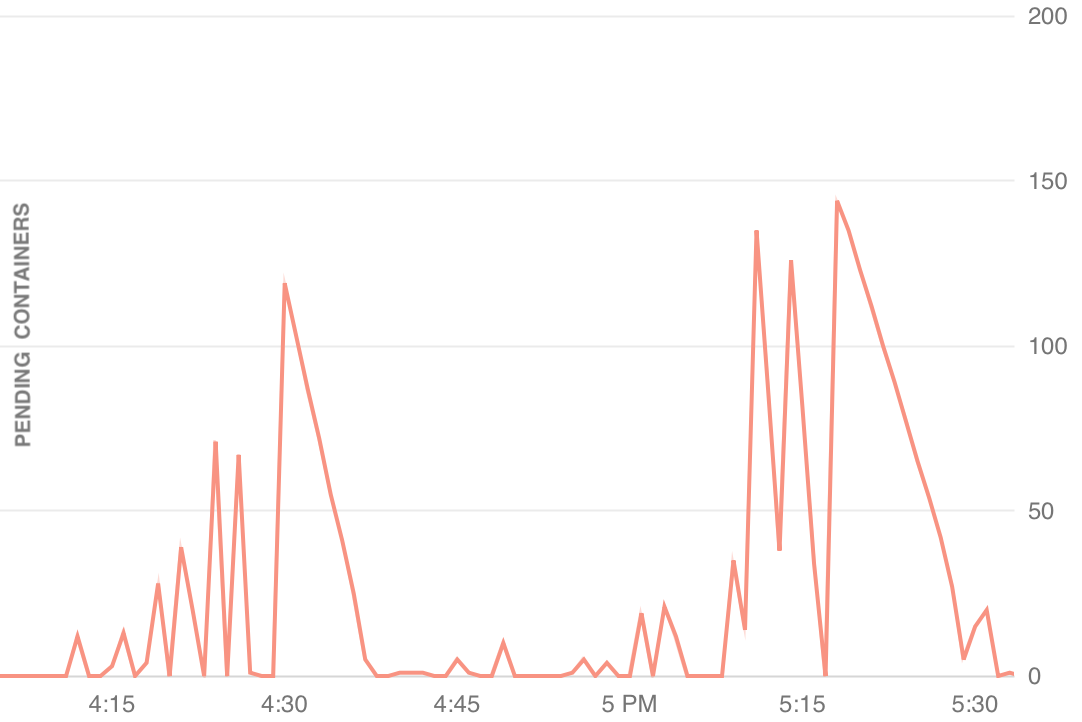
\includegraphics[height=80mm]{job-profile}
\caption{The number of YARN pending containers of the job executed in a cluster with minimum configuration.}\label{fig:job-profile}
\end{figure}

\section{Test set I}
We are going to test the autoscaler with three tests regarding the scaling factor: we will see the behaviour when he tries to satisfy immediately all the resource requests and in the case when it creates new resources more prudently. The base environment is the following:
\begin{itemize}
	\item Only 1 job in the cluster, as described in the previous section, with spare workload spikes.
	\item Downscaling disabled
	\item Timeout is 60 seconds
\end{itemize}
The only variable in this settings is the scaling factor; specifically, we are going to test with these three values:
\begin{enumerate}
	\item 1.0, it satisfies immediately each resource request
	\item 0.5, it satisfies immediately the half of resource requests
	\item 0.2, it satisfies immediately one-fifth of resource requests
\end{enumerate}

\subsection{High scaling factor}
In this test we are going to analyze the autoscaler behaviour with an aggressive configuration, satisfying immediately all the resource requests. In the Figure~\ref{fig:high-size} we can see the number of worker nodes during the execution: at the beginning, the scaling-up action is not really steep because of the processing of medium-size tables. After around 30 minutes we have the first two big tables to process and, for this reason, we have a big step to 20 and then to 26 nodes. Without downscaling for sure from this moment in advance we are going to be in an over-provisioned state. The significant number of nodes allows the cluster to immediately schedule each task, except at the end, when we have the biggest table to process: in this case we need to add just a few nodes.

\begin{figure}
\centering
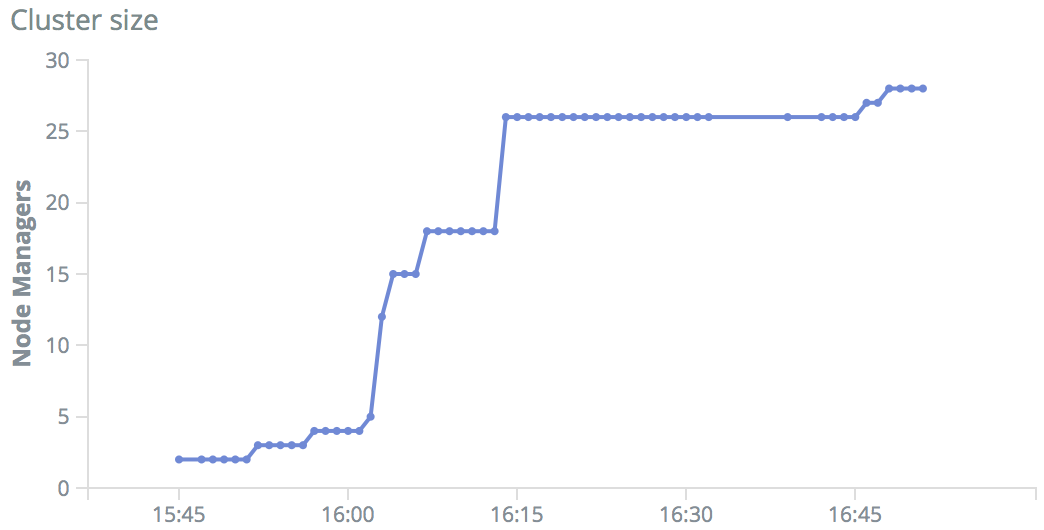
\includegraphics[height=80mm]{high-size}
\caption{The number of Node Managers during the execution of the production job in an autoscaled cluster with high scaling factor.}\label{fig:high-size}
\end{figure}

At this point, we could analyze the configuration performances looking at Pending Memory and Available Memory evolution, respectively in the Figure~\ref{fig:high-p-memory} and Figure~\ref{fig:high-a-memory}.

\begin{figure}
\centering
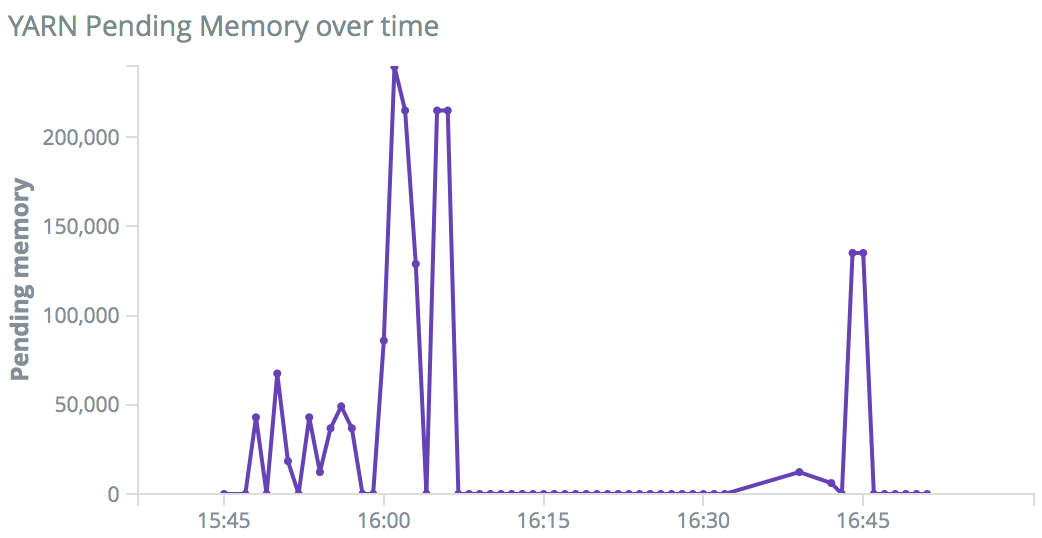
\includegraphics[height=80mm]{high-p-memory}
\caption{The evolution of \textit{Pending Memory} during the execution of the production job in an autoscaled cluster with high scaling factor.}\label{fig:high-p-memory}
\end{figure}

\begin{figure}
\centering
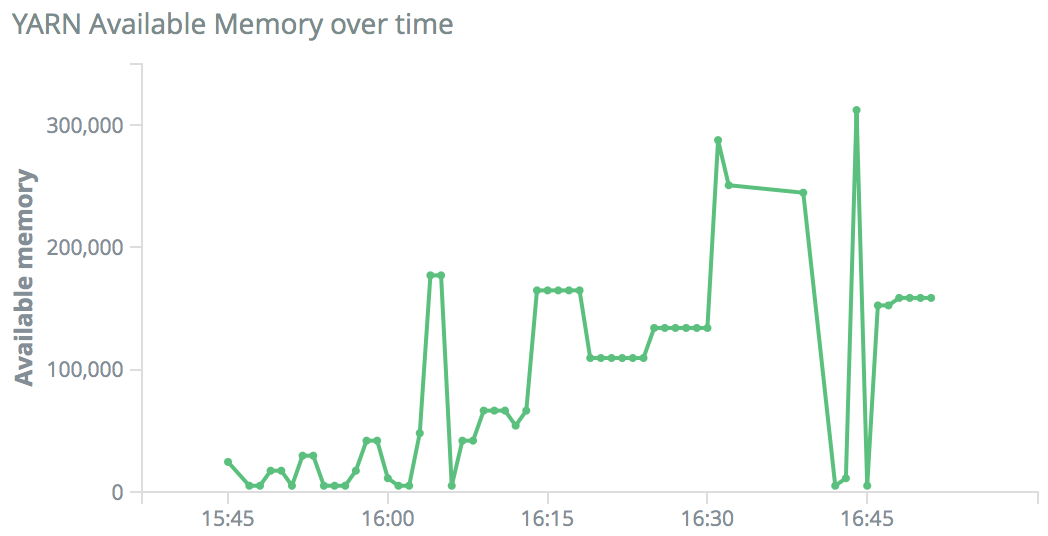
\includegraphics[height=80mm]{high-a-memory}
\caption{The evolution of \textit{Available Memory} during the execution of the production job in an autoscaled cluster with high scaling factor.}\label{fig:high-a-memory}
\end{figure}

The graph about the Pending Memory is really easy to understand, being really similar to the graph showing the Pending Containers evolution. We can see, again, the different resource requests based on small, medium or big table processing. In the graph about the Available Memory, we can clearly see that we have the over-provisioning problem: almost always we have available memory, even when there is no pending memory. Of course, this result is heavily biased from the absence of downscaling but, in any case, it happens what we have already discussed in the job analysis section: being more or less "late", due to the heuristics-based design and overhead introduced for Node Manager initialization, we allocate a lot of resources that are no longer needed. We can observe this fact especially at the very beginning of the job, dealing with medium-size tables: in theory we should have only a spike, corresponding to new nodes allocated but still not used; practically, we continue to add nodes to satisfy each incoming request and the available memory signal is always greater than zero.

In the Figure~\ref{fig:high-cost} we can analyze costs: in about 50\% of cases, we spend between 1.3\$ and 1.9\$, about 70\% of saving in terms of money. In the worst case, we spend about 2.35\$ (55\% savings) and in the luckiest case about 1\$ (80\% savings). 

\begin{figure}
\centering
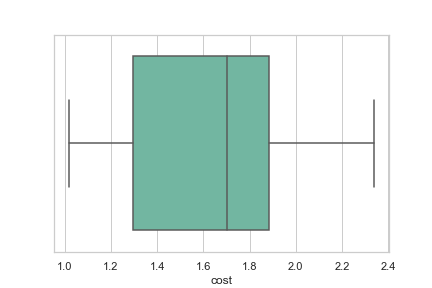
\includegraphics[height=80mm]{high-cost}
\caption{The costs distribution after 50 executions of the production job in an autoscaled cluster with high scaling factor.}\label{fig:high-cost}
\end{figure}

The results in terms of costs are quite promising but, in this case, we should focus more on duration performances, in Figure~\ref{fig:high-duration}. In the 50\% of cases, we have a duration between 4600 seconds (1 hour and 16 minutes) and 5000 (1 hour and 23 minutes). Of course, the new configuration can never beat the current production result, unless this last one leads to a heavy under-provisioning. But, in general, we could conclude that the performances are quite bad: in the worst case the job it is even 60\% slower. In the luckiest cases the job is only 10 minutes slower (18\% worse) but they are rare. A really high number of P-VM is a serious problem with reliability.

\begin{figure}
\centering
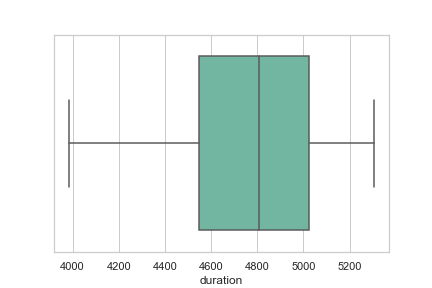
\includegraphics[height=80mm]{high-duration}
\caption{The duration distribution after 50 executions of the production job in an autoscaled cluster with high scaling factor.}\label{fig:high-duration}
\end{figure}

\subsection{Medium scaling factor}
In this test we are going to analyze the autoscaler behaviour with a balanced configuration, satisfying only half of the estimated resources. In the Figure~\ref{fig:high-size} we can see the number of worker nodes during the execution: immediately we can see the difference with respect to the case before because no additional nodes are added to process medium-size tables. After 30 minutes we have, again, a moderate scaling up to 10 nodes. We could go for over-provisioned again in this case, but with much fewer resources deployed; we can say more analyzing the memory graph in a while. An interesting thing to notice here is the impact of preemption: at the beginning of the second part (at around 12:00), we can see that the number of nodes decreases for 1-2 minutes; it is actually the mechanism discussed in Paragraph \ref{preemptible_explain}, about the managed group of preemptible VMs. As before, we have another scaling-up action to handle the biggest table processing.

\begin{figure}
\centering
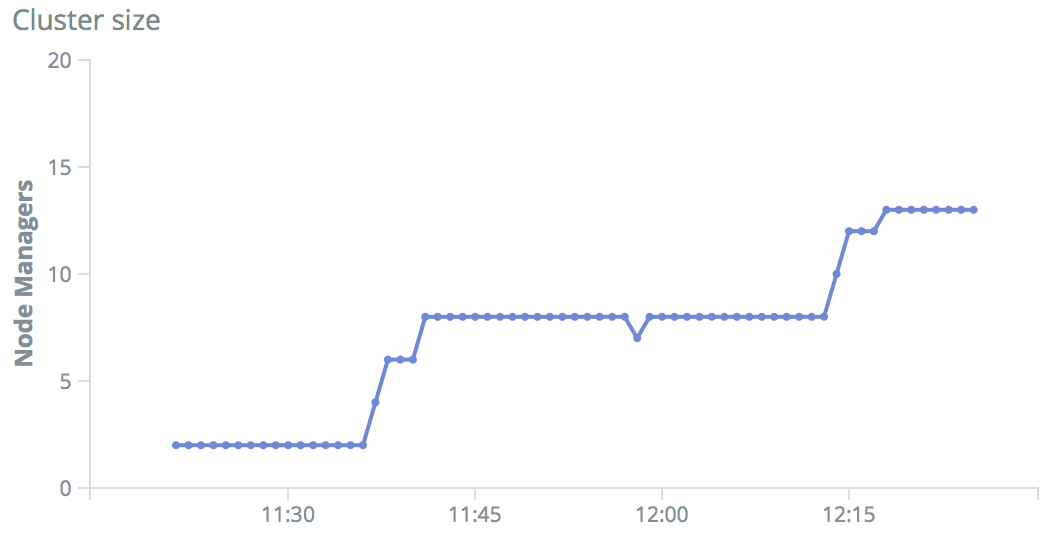
\includegraphics[height=80mm]{medium-size}
\caption{The number of Node Managers during the execution of the production job in an autoscaled cluster with medium scaling factor.}\label{fig:medium-size}
\end{figure}

Analyzing the memory-related metrics we can assess the goodness of a more conservative approach. In the Pending Memory graph, in Figure~\ref{fig:medium-p-memory}, we can see obviously the same pattern as before; from an absolute point of view, the quantity of pending memory is so much higher for obvious reasons. In addition, at the end of the job we can highlight two spikes instead of one: coming from a state where we had only 10 nodes instead of 26, the cluster does not find enough resources for the second biggest table (executed first) and the biggest one (executed almost at the end).
From the Available Memory graph, in Figure~\ref{fig:medium-a-memory}, we can assess that we clearly improved the over-provisioning issue. Most of the times are equal to zero, but we have to make clear two distinct cases:
\begin{enumerate}
	\item At the very beginning of the job we have pending memory greater than zero, so we are in a light under-provision situation; it is quite normal, knowing the configuration of the autoscaler 
	\item In the middle and at the very end of the job, we have both pending and available memory to zero, meaning that the cluster is perfectly sized (except for small negligible spikes).
\end{enumerate}

The only case when we still have over-provisioning is just after the 12:00 in the graph: for about 10 minutes we have pending memory equal to 0, but at the same time the available memory is not indifferent, reaching even 100.000 MB at some point. 

\begin{figure}
\centering
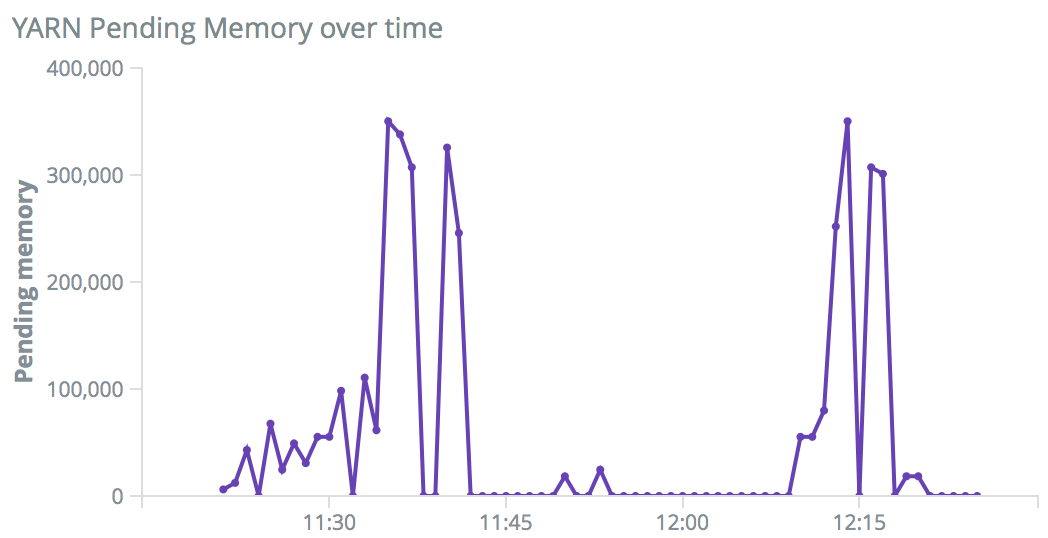
\includegraphics[height=80mm]{medium-p-memory}
\caption{The evolution of \textit{Pending Memory} during the execution of the production job in an autoscaled cluster with medium scaling factor.}\label{fig:medium-p-memory}
\end{figure}

\begin{figure}
\centering
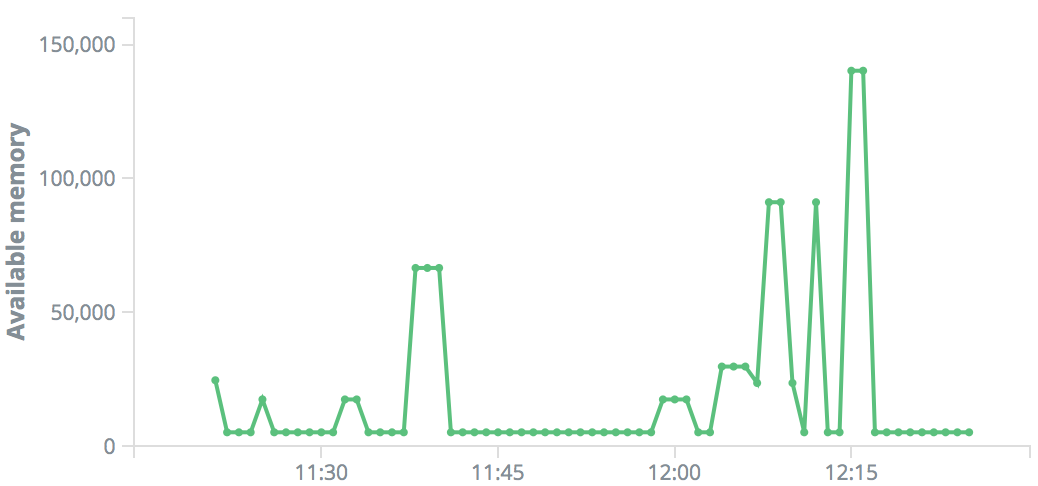
\includegraphics[height=80mm]{medium-a-memory}
\caption{The evolution of \textit{Available Memory} during the execution of the production job in an autoscaled cluster with medium scaling factor.}\label{fig:medium-a-memory}
\end{figure}

Analyzing the costs in the Figure~\ref{fig:medium-cost}, we can see that in about 50\% of cases we spend between 1.3\$ and 1.4\$, (about 75\% of saving in terms of money), that is a slight improvement with respect to the previous case. Where we can see a clear-cut improvement is the worst case: we spend about 1.6\$ (70\% savings), practically the most probable result in the previous case. 

\begin{figure}
\centering
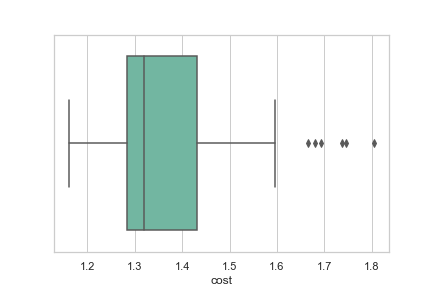
\includegraphics[height=80mm]{medium-cost}
\caption{The costs distribution after 50 executions of the production job in an autoscaled cluster with medium scaling factor.}\label{fig:medium-cost}
\end{figure}

We have already verified substantial improvements with respect to before but, in Figure~\ref{fig:medium-duration}, we can see that duration results are dramatically better: in the 50\% of cases we have a duration between 4100 seconds (1 hour and 8 minutes) and 4450s (1 hour and 14 minutes). In the worst case, the job is executed in 4850s (1 hour and 20 minutes), meaning the 45\% slower: it is not a really good result, but much better with respect to the previous case. In the most favourable cases, on the contrary, the job is only 3 minutes slower (5\% worse), that is an excellent result.

\begin{figure}
\centering
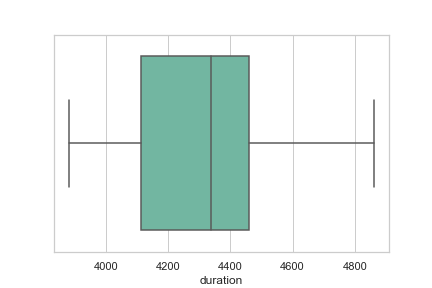
\includegraphics[height=80mm]{medium-duration}
\caption{The duration distribution after 50 executions of the production job in an autoscaled cluster with medium scaling factor.}\label{fig:medium-duration}
\end{figure}

\subsection{Low scaling factor}
In this test we are going to analyze the autoscaler behaviour with a really conservative configuration, satisfying only one-fifth of estimated resources. In the Figure~\ref{fig:high-size} we can see the number of worker nodes during the execution: it is really low, using at maximum only 4 nodes for most of the time, scaling to 7 nodes at the end for the two big tables as usual. Of course, this approach is really resource-saving but there is the risk to have a cluster under-provisioned.

\begin{figure}
\centering
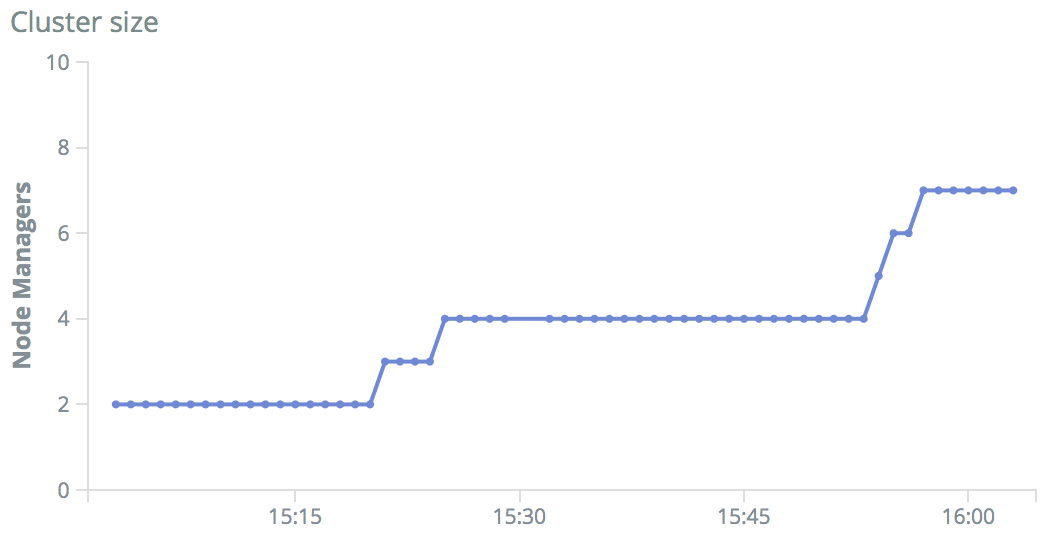
\includegraphics[height=80mm]{low-size}
\caption{The number of Node Managers during the execution of the production job in an autoscaled cluster with low scaling factor.}\label{fig:low-size}
\end{figure}

Taking a look at the Figure~\ref{fig:low-p-memory} and Figure~\ref{fig:low-a-memory} we can reason about the under-provisioning aspect.

\begin{figure}
\centering
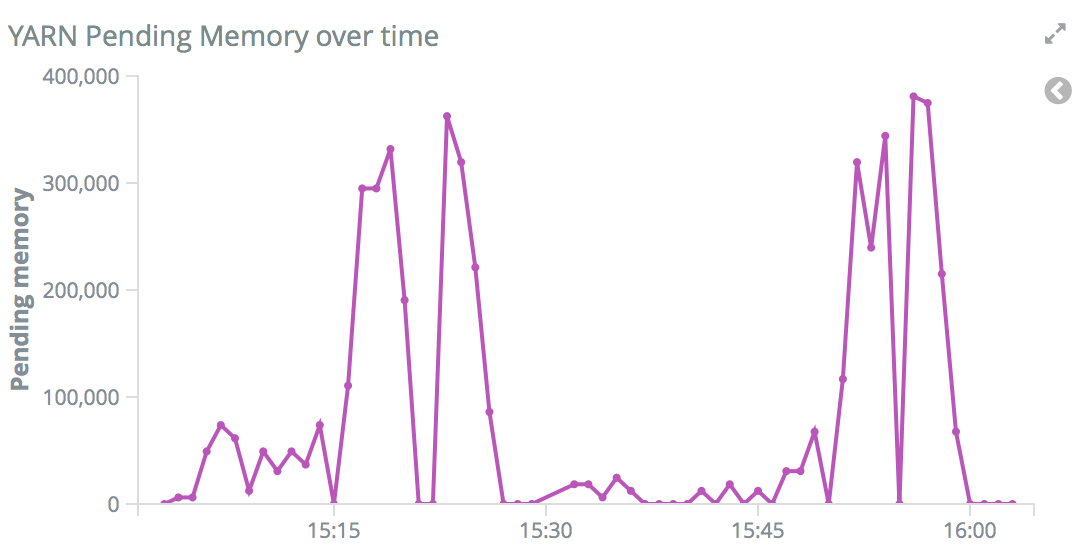
\includegraphics[height=80mm]{low-p-memory}
\caption{The evolution of \textit{Pending Memory} during the execution of the production job in an autoscaled cluster with low scaling factor.}\label{fig:low-p-memory}
\end{figure}

\begin{figure}
\centering
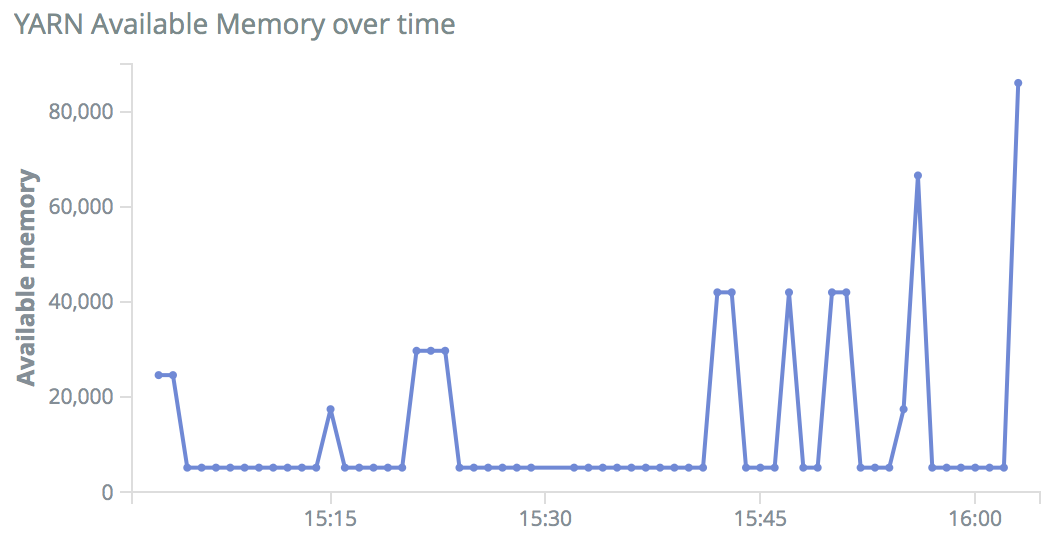
\includegraphics[height=80mm]{low-a-memory}
\caption{The evolution of \textit{Available Memory} during the execution of the production job in an autoscaled cluster with low scaling factor.}\label{fig:low-a-memory}
\end{figure}

We have quite the opposite situation with respect to the first test, with scaling factor equal to 1: the available memory is quite always equal to 0, except for the minutes when a scaling-up action was triggered. About the pending memory evolution, the graph is quite the same to the previous case but the under-provisioning issue is slightly worse in this case:
\begin{enumerate}
	\item At the very beginning of the job we have pending memory greater than zero but, with respect to the previous case, now we are in a not indifferent under-provision situation, with pending memory quite always over 50.000 MB.
	\item In the middle of the job, where the cluster was perfectly sized in the previous case, we have a light under-provisioning situation but still acceptable, the pending memory is constantly greater than zero but with low values.
\end{enumerate}

As expected, the costs are really low in this case, as shown in Figure~\ref{fig:low-cost}. In the half of the cases they are included in a range from 0.85\$ to 0.95\$, that is a really low cost: it is an 83\% cut! In the worst case, where the expenditure is around 1.1, the costs are even better than 95\% of the results obtained with the previous configuration.

\begin{figure}
\centering
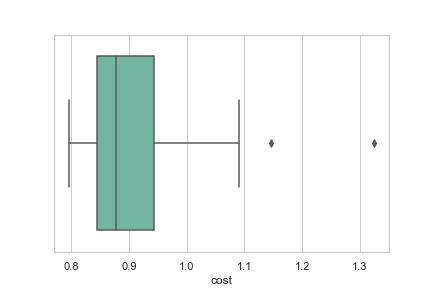
\includegraphics[height=80mm]{low-cost}
\caption{The costs distribution after 50 executions of the production job in an autoscaled cluster with low scaling factor.}\label{fig:low-cost}
\end{figure}

The duration performances are really good: in Figure~\ref{fig:low-duration} we can find the first and the third quartile corresponding respectively to around 3800s (1 hour and 3 minutes) and 3900s (1 hour and 5 minutes), only 15\% worse. Even under this point of view, the worst case is better than 75\% of all cases in the previous configuration: 4100s seconds (1 hour and 8 minutes). It is clear that the usage of a low quantity of preemptible VMs is the key to improve performances.

\begin{figure}
\centering
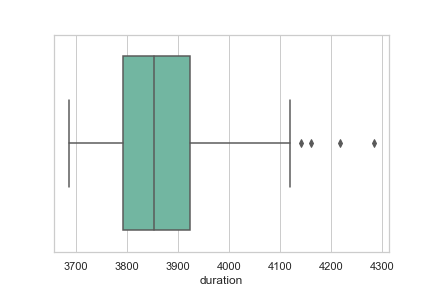
\includegraphics[height=80mm]{low-duration}
\caption{The duration distribution after 50 executions of the production job in an autoscaled cluster with low scaling factor.}\label{fig:low-duration}
\end{figure}

\subsection{Conclusions}
As expected during the job analysis, in this case, an autoscaler that try to tightly follow the workload signal is not worth it, and the downscaling disabled make everything worse. Figure ~\ref{fig:test1-cost-comparison} shows us the comparison between the three configurations in terms of costs. The result is quite expected: with fewer nodes we spend less money. We cannot consider another evidence in the comparison: the length of the box and whiskers in the graph. We can clearly see the effect of preemptible VMs usage and how they impact the job performances. Using a considerable number of P-VMs, we increase the probability of preemption: as a consequence of that, there is so much randomness in the result. In the most unlucky case, the preemption could heavily degrade performances, provoking the re-execution of some tasks, taking alive the cluster for more time and definitely spend more money. 

\begin{figure}
\centering
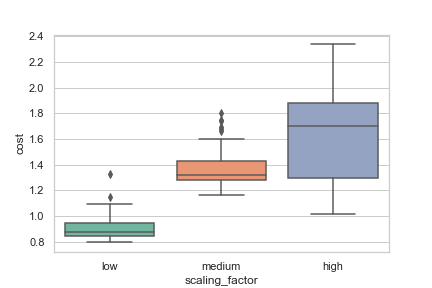
\includegraphics[height=80mm]{test1-cost-comparison}
\caption{The cost comparison between the three different autoscaler configuration, with downscaling disabled.}\label{fig:test1-cost-comparison}
\end{figure}

The preemption effect is still visible in the duration comparison in Figure~\ref{fig:test1-duration-comparison}, where the box and whisker length gradually increases according to the scaling factor. Paradoxically, the best result is obtained with the more conservative configuration, where we have only a small quantity (or even not at all) of failed tasks.

\begin{figure}
\centering
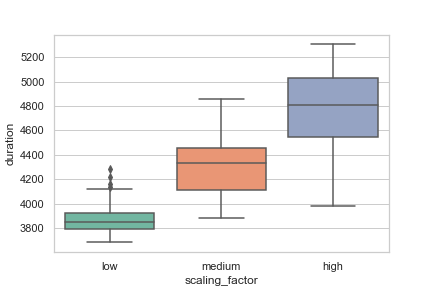
\includegraphics[height=80mm]{test1-duration-comparison}
\caption{The duration comparison between the three different autoscaler configuration, with downscaling disabled.}\label{fig:test1-duration-comparison}
\end{figure}

At end of this test set, we have learned that:
\begin{enumerate}
	\item A scaling factor equal to 1.0 make the autoscaler too flexible and it is not the best configuration in this case when we have isolated spikes for a few minutes.
	\item A scaling factor equal to 0.2 is good but leads to under-provisioning. Enabling the downscaling with this scaling factor does not make sense.
\end{enumerate}

From here, we are going to do a step further, enabling the downscaling with scaling a factor equal to 0.5, in order to solve the over-provisioned state detected during our last analysis.

\section{Test set II} \label{test-set-ii}
In this test set, we capitalize on what we have learned in the previous tests and try to do better enabling the downscaling feature. Specifically, this is the base environment:
\begin{itemize}
	\item Only 1 job in the cluster, the same as before.
	\item Downscaling enabled
	\item Scaling factor equal to 0.5
	\item Timeout is 120 seconds
\end{itemize}
The only variable in this settings is the Graceful Decommissioning Timeout, as explained in Paragraph \ref{yarn_intro}; specifically, we are going to test with these two values:
\begin{enumerate}
	\item 120s
	\item 300s
\end{enumerate}

In general, the behaviour of the autoscaler is the same for both configurations. The most important thing here is to validate the reliability of these two configurations. In order to have a general overview of the autoscaler behaviour, in Figure~\ref{fig:down-size} we can see the size of the cluster during the job execution. For most of the time, the cluster size is equal to 2, except for that moment when the processing of medium and big-size tables.  

\begin{figure}
\centering
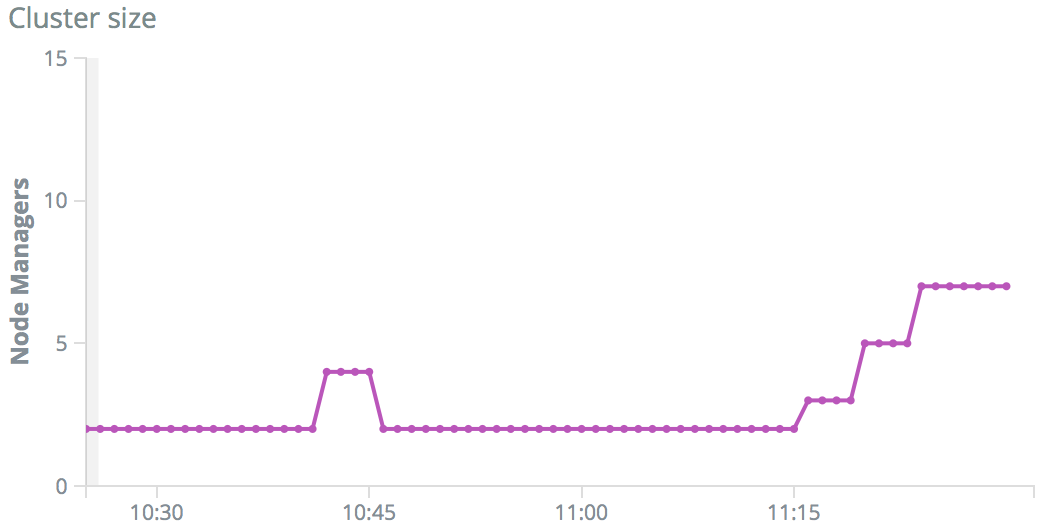
\includegraphics[height=80mm]{down-size}
\caption{The number of Node Managers during the execution of the production job in an autoscaled cluster with low scaling factor and downscaling enabled.}\label{fig:down-size}
\end{figure}

Figure~\ref{fig:down-pa-memory}, about the evolution of the Pending and Available Memory metrics, shows a really similar behaviour with respect to the autoscaler configuration with a low scaling factor: indeed, we can notice a light under-provisioning state at the beginning and in the middle of the job execution, as explained before.

\begin{figure}
\centering
	\begin{subfigure}[b]{0.4\textwidth}
    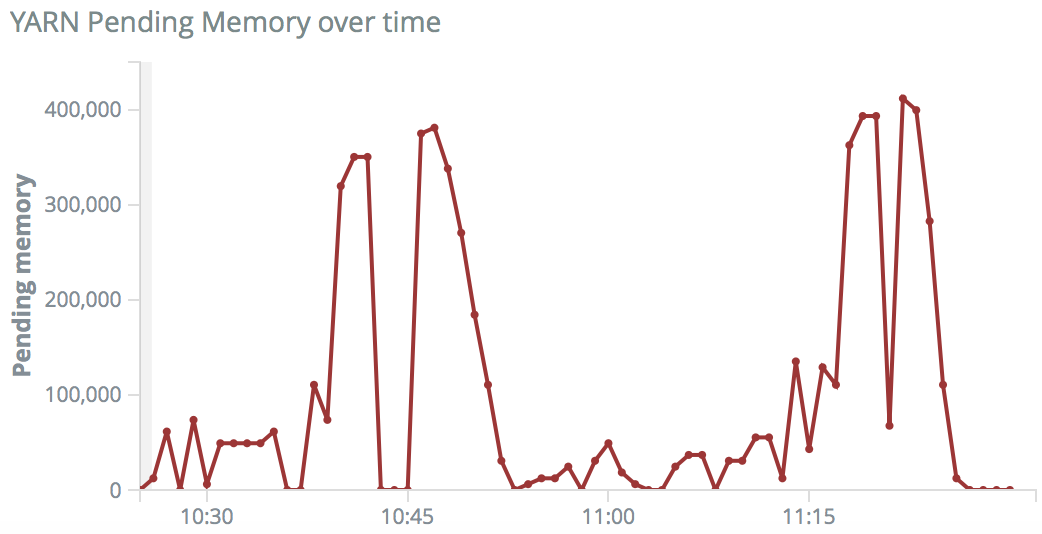
\includegraphics[height=30mm]{down-p-memory}
	\caption{Pending memory}\label{fig:down-p-memory}
  \end{subfigure}
	%%%
	\begin{subfigure}[b]{0.4\textwidth}
	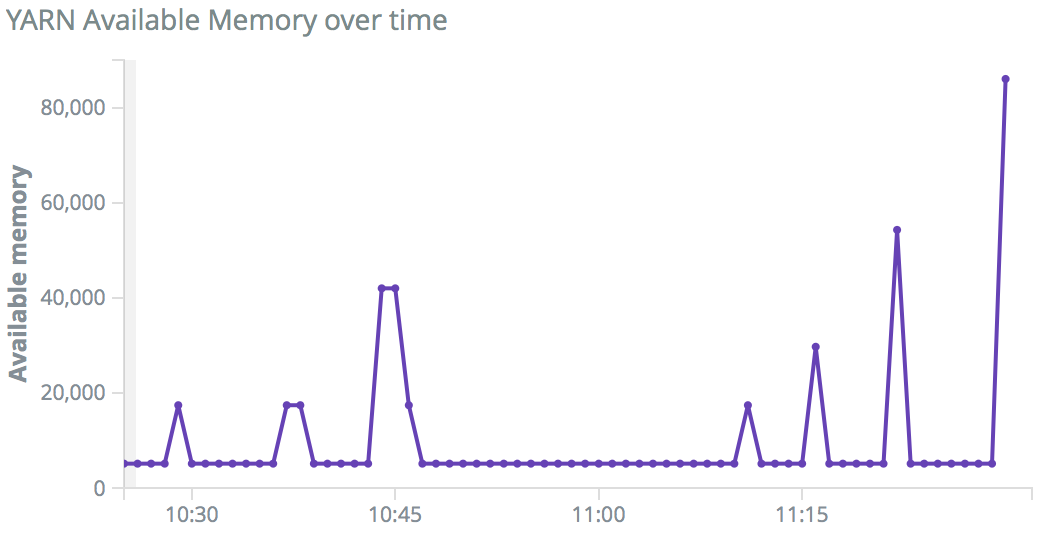
\includegraphics[height=30mm]{down-a-memory}
	\caption{Available memory}\label{fig:down-a-memory}
	\end{subfigure}
	\caption{The evolution of \textit{Pending Memory} and \textit{Available Memory} during the execution of the production job in an autoscaled cluster with fast graceful decommissiong.}\label{fig:down-pa-memory}
\end{figure}

\subsection{Fast decommissioning}
The first attempt is to understand if 2 minutes are sufficient in order that the graceful decommission is effective. After 50 execution of the same test, the results are summarized in Table \ref{table:fast-down}

\begin{table}[]
\centering
\begin{tabular}{|c|c|}
\hline
\multicolumn{2}{|c|}{50 executions} \\ \hline
Success          & Failure          \\ \hline
31               & 19               \\ \hline
\end{tabular}
\caption{}\label{table:fast-down}
\end{table}

The results are not so good: in the 38\% of the cases, the job failed. Analyzing the Spark driver logs, we could realize that the most common error is \textit{org.apache.spark.shuffle.FetchFailedException}: other tasks tried to fetch data from a node that no longer exists. It is possible to see this error at least one time in \textit{every} job log but, in the most unlucky cases, it was thrown multiple times and this led to job failure. In few words, with this configuration, when a node is marked as "decommissioning", it has only 2 minutes not only to complete all the running tasks but even to accept all the fetch data requests in order to complete the shuffling. From our results, we can conclude that 2 minutes is a too small timeout to have a good reliability level.

Before passing directly to the next test, we analyze the time and cost performances, especially making a comparison with the best configuration so far, with the low scaling factor. The Figure~\ref{fig:fast-down-cost} shows us that with the downscaling we improved again under the costs point of view: in the 75\% of the case we spend less than 0.85\$ and, in the 25\% case we even go under the 0.80\$. It means an 85\% cut with respect to the production case!

\begin{figure}
\centering
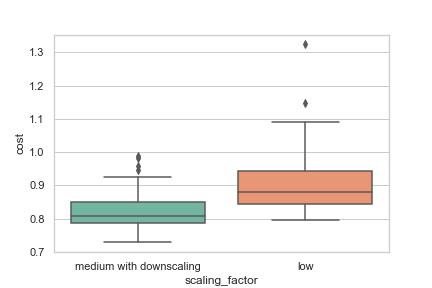
\includegraphics[height=80mm]{fast-down-cost}
\caption{The cost comparison between the conservative configuration (no downscaling) and that one with 2 minutes as gracefully decommissioning.}\label{fig:fast-down-cost}
\end{figure}

In view of the above, the results showed in the Figure~\ref{fig:fast-down-duration} are quite surprising: in general, the duration distribution is higher, even if we have spent less money. This is the clear sign of the effectiveness of downscaling in terms of resource savings and over-provisioning avoidance, but at the time it introduces the possibility to degrade time performances. The 62\% of the jobs, even if they succeeded, they wasted a considerable time interval (some more, some less) to recompute some tasks. We cannot see the impact of this on the cost performances because the failure handling process is executed with a limited number of nodes (because of downscaling, of course) that, in the case of preemptible VMs usage, introduce derisory costs. 

\begin{figure}
\centering
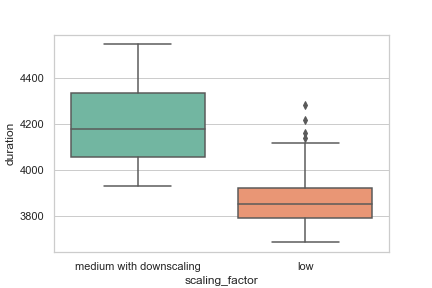
\includegraphics[height=80mm]{fast-down-duration}
\caption{The duration comparison between the conservative configuration (no downscaling) and that one with 2 minutes as gracefully decommissioning.}\label{fig:fast-down-duration}
\end{figure}

\subsection{Slow decommissioning}
In this second attempt, we will try to improve the previous performances setting to 5 minutes the graceful decommission timeout. After 50 execution of the same test, the results are summarized in Table \ref{table:slow-down}.

\begin{table}[]
\centering
\begin{tabular}{|c|c|}
\hline
\multicolumn{2}{|c|}{50 executions} \\ \hline
Success          & Failure          \\ \hline
41               & 9               \\ \hline
\end{tabular}
\caption{}\label{table:slow-down}
\end{table}

We hugely improved the reliability performances: in this case, we have only 18\% of job failure. Of course, it is not a fantastic result but we should remember that we have to accept this if we want to maximize cost savings using the preemptible VMs. Then, It would be up to the user, based on his needs, to set a configuration in order to balance reliability and expenditure.

In Figure~\ref{fig:slow-down-cost} a comparison between the two autoscaler with graceful decommission and the conservative configuration without downscaling. Even if we take the nodes alive for a longer time, we improved again the costs performances: in almost 100\% of the cases, we are between the 0.70\$ and 0.80\%, with a saving up to 87\% with respect to the production case. 

\begin{figure}
\centering
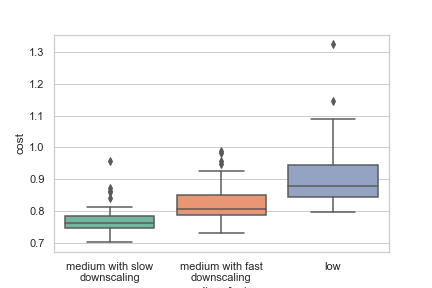
\includegraphics[height=80mm]{slow-down-cost}
\caption{The cost comparison between the conservative configuration (no downscaling), 2 minutes and 5 minutes as gracefully decommissioning.}\label{fig:slow-down-cost}
\end{figure}

The result showed in Figure~\ref{fig:slow-down-duration} is really interesting: we did not improve the time performances so much but it is impossible not to notice the huge length of the whiskers. They cover the whole time range merging the two configurations that we took as reference so far: in the 25\% of the cases we have similar performances to the conservative approach, in 50\% we have slightly better performances with respect to the configuration with 2 minutes as graceful decommission timeout but we could notice that in some cases (the end of the upper-whisker) we obtained even worse result. A reasonable interpretation of this result could be the following: with no doubts, as the previous table confirms, we have improved the reliability performances. This fact could be visible in the fact that, in a considerable portion of the results, we obtained really good results, similar to the configuration without downscaling. But the real question to ask is: how could be possible that, in some cases, we obtained worse performances with respect to the fast downscaling? The answer could be tricky, but the reason is, again, because we improved reliability performances. With a longer graceful decommission timeout we have decreased the number of failures, but we did not solve the problem completely, as Table \ref{table:slow-down} remembers. Decreasing the number of job failures, we kept alive more jobs with many task failures and, as a consequence of that, many of them drastically slowed down due to failure handling procedures. 

\begin{figure}
\centering
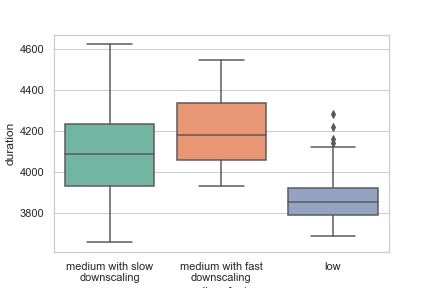
\includegraphics[height=70mm]{slow-down-duration}
\caption{The duration comparison between the conservative configuration (no downscaling), 2 minutes and 5 minutes as gracefully decommissioning.}\label{fig:slow-down-duration}
\end{figure}

\subsection{Conclusions}
Downscaling is very advantageous and brings real benefits from an economic point of view. However, it can turn out to be a double-edged sword: by setting a graceful decommission timeout too short, we can have serious reliability problems. Even with more reasonable timeouts, we do not completely eliminate the problems that can lead to job failures, but the administrator can find a good compression based on the duration of the job and time constraints. In the case of the job analyzed so far, because of its characteristics, it is more convenient to use a conservative configuration without downscaling, since there are no long workloads that would bring to a large cluster size from which it is no longer possible to go back. Indeed, for this case, we could save around 0.10\$ but with the risk to execute the job (at least) twice, destroying cost optimization due to downscaling.

\section{Google autoscaler comparison}
In this section we are going to assess if our autoscaling design leads to an improvement with respect to the Google version, our principal starting point and reference. For this reason, we will do comparison tests to evaluate differences between the two versions. Of course, we will setup the Google autoscaler treasuring what we have learned about the previous tests and the job; we will go for a conservative configuration, the best one for the kind of job we are dealing with. As we know from its analysis in the state of the art, in Equation \ref{eq:delta_n}, even in the Google implementation we have a scaling factor variable that we could tune. Specifically, we will set these parameters in the configuration object:
\begin{itemize}
	\item \textit{dataproc:alpha.autoscaling.cooldown\_period} to "10m", that is the minimum value.
	\item \textit{dataproc:alpha.autoscaling.scale\_up.factor} to "0.2", as in conservative configuration.
	\item \textit{dataproc:alpha.autoscaling.graceful\_decommission\_timeout} to "5m", as we discussed in the last section.
\end{itemize}
Then we set other not really important parameters just to force the autoscaler to use only preemptible VMs.

At this point, we can immediately see the evolution of cluster size in Figure~\ref{fig:google-size}. The behaviour seems really coherent with we have seen so far: comparing this result with the cluster size in Figure~\ref{fig:down-size}, obtained with the low scaling factor, we could realize that the scaling decisions are quite identical. For this reason we will expect similar result both for costs and duration performances. One more important thing to notice it that, even if in the Google configuration the downscaling is enabled, it could not catch any moment when a downscaling is required. In general, this fact could be caused by two factors, as already discussed during its study in the state of the art analysis:
\begin{enumerate}
	\item The low reactivity of the Google implementation due to large timeout constraints. 
	\item The logic based on a raw average of resources.
\end{enumerate}
The combination of these two factors does not allow to isolate the time range when the need of downscaling is clear and, in addition, the "signs" of downscaling required, happening in the last metrics of the window for example, will be balanced out by the strong resources requests contained in the past but in the same window.

\begin{figure}
\centering
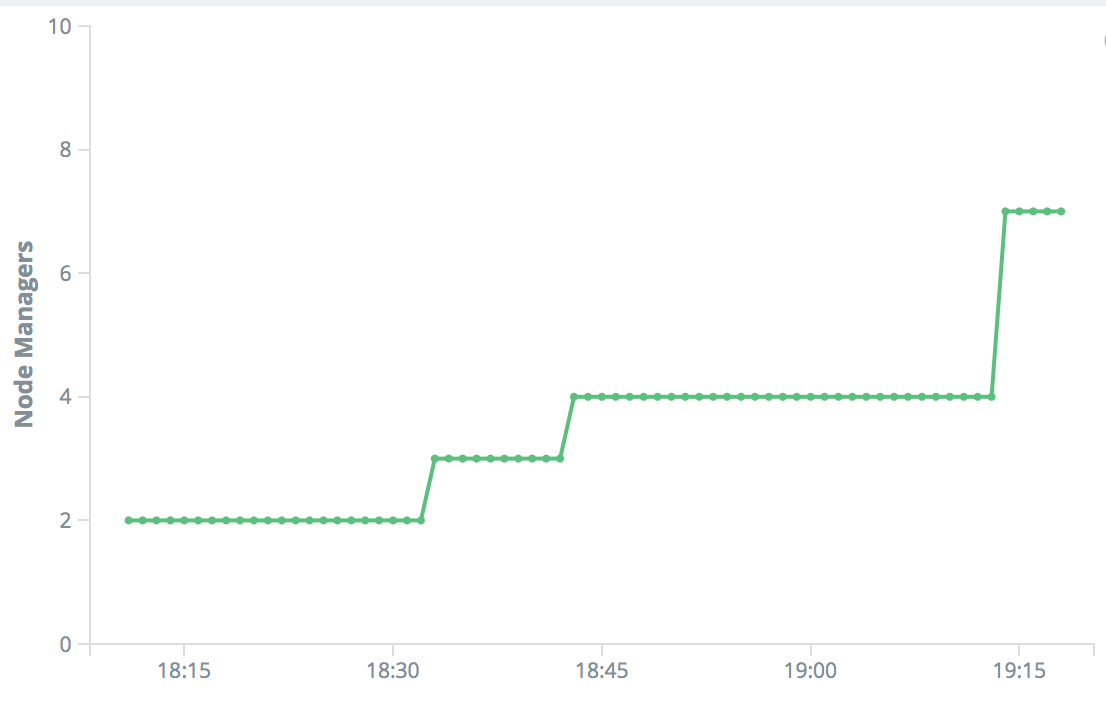
\includegraphics[height=80mm]{google-size}
\caption{The number of Node Managers during the execution of the production job in a cluster controlled by Google autoscaling mechanism.}\label{fig:google-size}
\end{figure}

Figure~\ref{fig:google-cost} is a comparison between the two best OBI configurations (with and without downscaling) and the Google version. There is no huge difference between these three cases but, more specifically, we can confirm the strong similarity with the conservative configuration. The larger variance, in the case of this last one, could be attributed to adverse conditions about preemption: during the execution of this test, in none of the 50 runnings clusters controlled by Google autoscaler we had a preemption event. 
After all, it is an expected result considering that the cluster size evolution are quite similar. The winner in this comparison is the configuration with downscaling, feature not exploited by the Google logic for the reasons explained just before. 

\begin{figure}
\centering
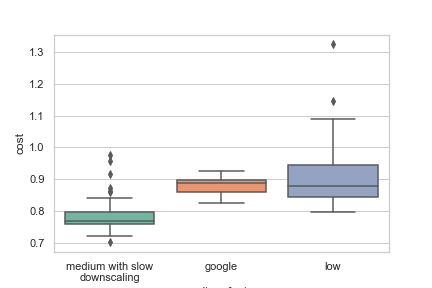
\includegraphics[height=80mm]{google-cost}
\caption{The cost comparison between the two best configurations and the autoscaler by Google (conservative configuration).}\label{fig:google-cost}
\end{figure}

In the Figure~\ref{fig:google-duration} we can assess the quality of the OBI autoscaler against the Google one. The performances of are quite similar: the duration distribution of the Google implementation is more similar to the "medium with downscaling" configuration, with a low variance in the distribution. The best one, in this case, is the OBI autoscaler with conservative configuration that provides a better result in the 50\% of the cases. 
\begin{figure}
\centering
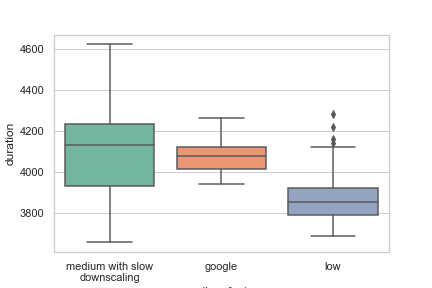
\includegraphics[height=80mm]{google-duration}
\caption{The duration comparison between the two best configurations and the autoscaler by Google (conservative configuration).}\label{fig:google-duration}
\end{figure}

\section{Custom job}
In all the analysis we have done so far, we always considered a job with high and short workload spikes. These characteristics were really favourable to the conservative configuration. We have just seen that, even if we enable the downscaling, the costs savings will be negligible. At this point, we are going to test a job with a different profile. We are looking for a job with a long, continuous high workload in the first part, and then a really low workload in the second half of the execution. Because of the absence of jobs with this profile in the work context, we will examine a modified version of the previous job. As in the original version, the code is essentially a \textit{for loop}. Remembering the Figure~\ref{fig:job-profile}, we will populate the list with only two table: the first one is that one corresponding to the highest spike on the right (between 5:15 and 5:30 in the graph), that we will call it "big table"; the second one is any table in the middle of the job execution, that we will call it "small table". The idea is using more times these two tables to build a job with characteristics we want. At the end of the day, the code will loop the following list of tables:
\begin{enumerate}
	\item Big table
	\item Big table
	\item Small table x15
\end{enumerate}

What we expect is that, even if it satisfies only 20\% of the estimated needed resources at each autoscaling action, the conservative autoscaler will satisfy completely the resource requests in many iterations due to the high workload for a long period. Actually, it is what we can visualize in Figure~\ref{fig:custom-size}. In this workload case the downscaling action is advantageous with no doubts: in the comparison in Figure~\ref{fig:custom-sizes} we can see that in the second part of the job a lot of useless nodes are kept alive, impacting negatively the costs. Then we have to notice the completely wrong behaviour of the Google autoscaler, as shown in Figure~\ref{fig:custom-google-size}: due to its problems explained in the previous paragraph, the logic added more nodes when the requests for resources was falling down. The result is that the cluster run with only 2 nodes to handle the big tables and with 6 nodes for small tables. We could expect bad performances, especially in the duration results. 

\begin{figure}
\begin{subfigure}{.5\linewidth}
\centering
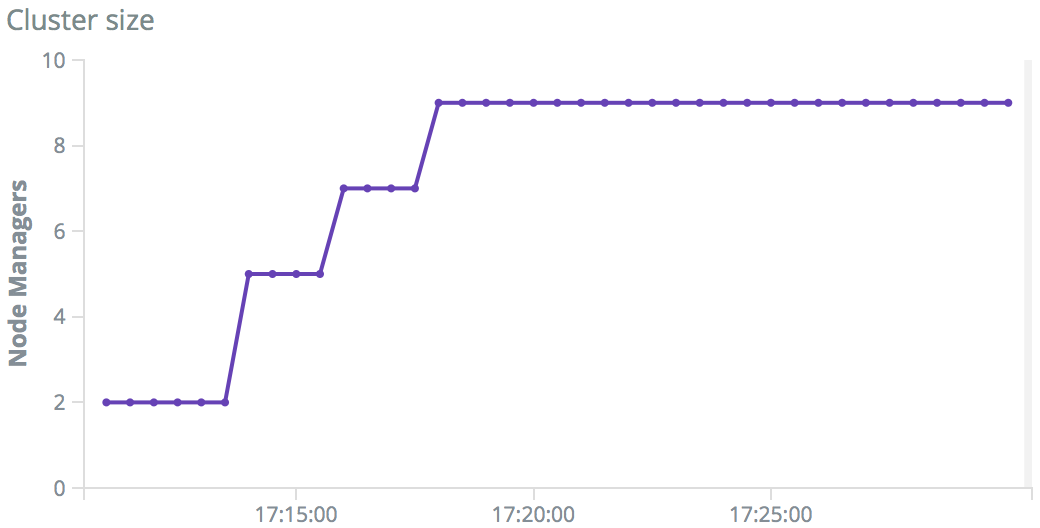
\includegraphics[height=30mm]{custom-size}
\caption{Conservative}\label{fig:custom-size}
\end{subfigure}%
\begin{subfigure}{.5\linewidth}
\centering
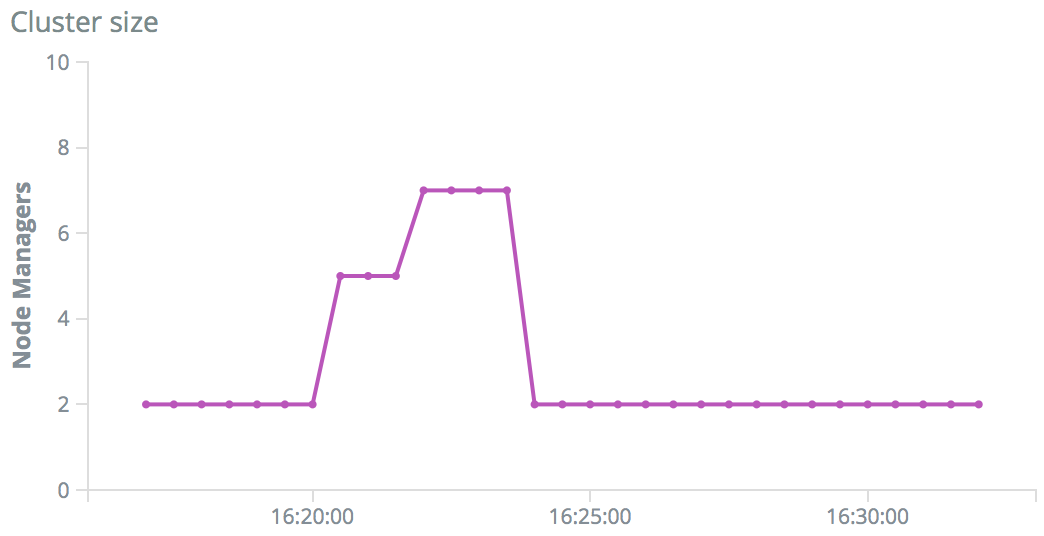
\includegraphics[height=30mm]{custom-down-size}
\caption{Medium, downscaling (5 min.)}\label{fig:custom-down-size}
\end{subfigure}\\[1ex]
\begin{subfigure}{\linewidth}
\centering
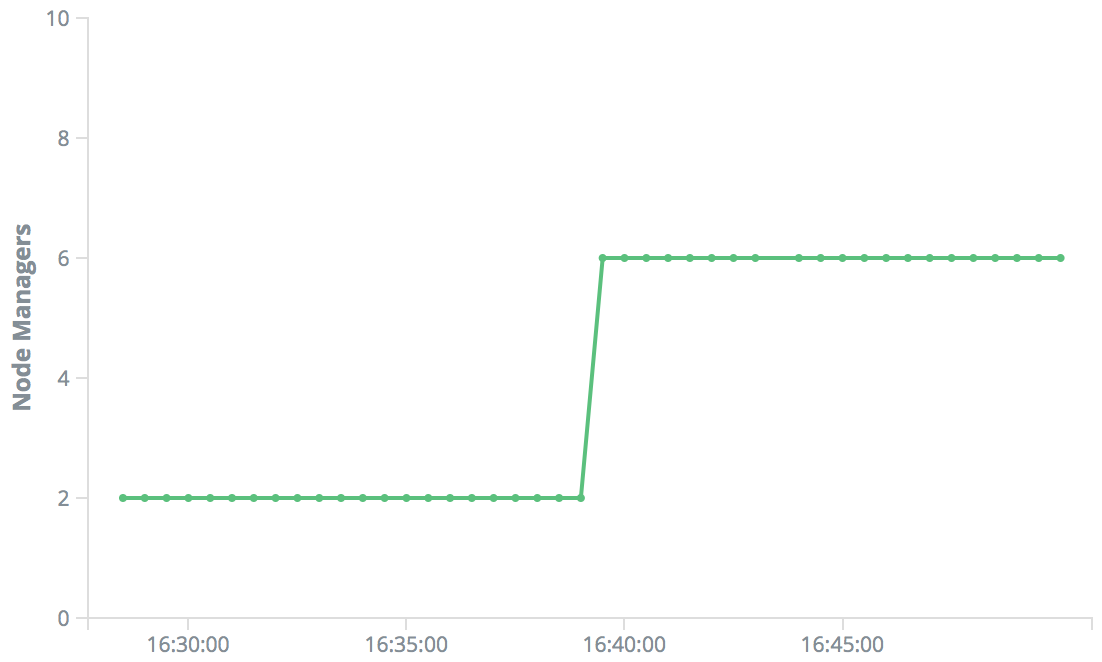
\includegraphics[height=30mm]{custom-google-size}
\caption{Google}\label{fig:custom-google-size}
\end{subfigure}
\caption{The \textit{Cluster size} comparison during the execution of the custom job, between the conservative configuration and the medium with downscaling one.}\label{fig:custom-sizes}
\label{fig:test}
\end{figure}

Finally, in the Figure~\ref{fig:custom-comparison} we can visualize the comparison between the three configurations in terms of expenditure and execution time. The graph about the latter one, in Figure~\ref{fig:custom-duration}, is not really interesting: as we have seen before, the downscaling introduces reliability problems, spreading the distribution in the box-plot: in more than 25\% of the case the OBI autoscaler with downscaling goes better but in some other cases could be worse; in the most of cases, the time duration is quite similar, overall. In this analysis the Google autoscaler is the worst, with all the performances comparable to the worst cases of the OBI autoscaler with medium scaling factor; this result is not surprising after we checked that all the scaling decisions taken by the Google autoscaler were wrong and out of time. The advantages of downscaling, for this kind of workloads, are visible in practice in the Figure~\ref{fig:custom-cost}: in the 75\% of the cases, even if we have to run the job twice, we will get a cost inside the conservative configuration distribution. Of course, there are still improbable cases where we could spend more but they are both with low probability to happen and in case the difference in terms of money is not too much. Therefore, we can conclude that we have to deal with these job types, it is better to go for a configuration with a medium/high scaling factor and downscaling enabled. This time the Google autoscaler takes the second place, but probably by chance: it simply scaled up only for the last minutes of the job, maintaining 6 nodes for a shorter period with respect the others (and when they were no longer needed).

\begin{figure}
\centering
	\begin{subfigure}[b]{0.4\textwidth}
    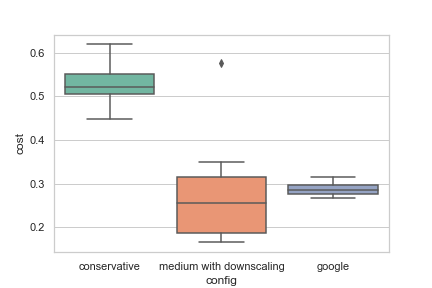
\includegraphics[height=45mm]{custom-cost}
	\caption{The cost comparison.}\label{fig:custom-cost}
  \end{subfigure}
	%%%
	\begin{subfigure}[b]{0.4\textwidth}
	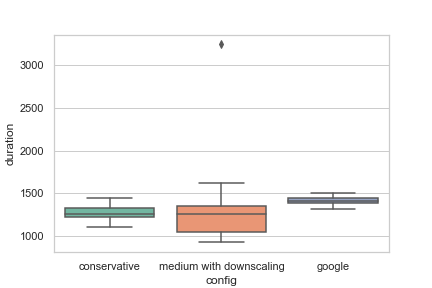
\includegraphics[height=45mm]{custom-duration}
	\caption{The time execution comparison}\label{fig:custom-duration}
	\end{subfigure}
	\caption{The cost and duration comparison during the execution of the custom job, between the conservative configuration, the medium with downscaling and the google implementation.}\label{fig:custom-comparison}
\end{figure}


\chapter{Conclusion}
All the tests executed so far have been really useful to understand strengths and weakness of the autoscaler and how to configure it in the future. In general terms, we can conclude:
\begin{enumerate}
	\item The scaling factor is the most important parameter when we think about performances. Depending on the job profile, it is useless to satisfy immediately all the estimated needed resources, therefore, an high value of this is not synonymous with better performances.
	\item Downscaling is easy in logic, really difficult in practice. Removing nodes during job execution has a significant negative impact on performances. The key to minimize this kind of issues is the Graceful Decommissioning feature. 
	\item There is no closed formula to determine the Graceful Decommissioning timeout. Longer is better, of course. The administrator should find a reasonable time to allow tasks completion and shuffling and limit costs at the same time.
	\item Despite the graceful decommissioning, we cannot completely solve all the reliability problems. For this reason, sometimes it is better a conservative approach with downscaling disabled.
	\item A thoughtful choice of the autoscaler timeout should not be neglected because it influences how much overhead the autoscaling logic introduces in the cluster lifetime. For example, a really short timeout for workload with high variability in the short period leads to bad performances, because of the continuous resize operations that make the cluster unstable.
\end{enumerate}

\section{Issues}
Software configuration is another important step during cluster creation. In the OBI context, where the final user does not care about the cluster, this process is a responsibility of the infrastructure administrator that will care about the OBI configuration. In the Google Cloud Platform, there are two possible ways to accomplish this task:
\begin{enumerate}
	\item Initialization script
	\item Custom images
\end{enumerate}
In the case of the \textit{initialization script}, we could specify the path of a bash script that will be executed in each node of the cluster after the cluster is set up. We can leverage this scripts to download, install and configure dependencies. The drawback is that this process requires time, depending on the size and quantity of packages we need. During the autoscaler testing we realized that, after a scaling up action, the new nodes took about 6 minutes before being available in the YARN context, ready to accept resource allocation requests. It is clear this huge overhead destroys the autoscaler effort, making his job pointless. Therefore, we moved for the second option, using the \textit{custom images}. The Google Cloud Platform allows us to build, starting from the original Dataproc image for Compute Engine, a custom version of it, in order to have an image with pre-installed packages. This is an important tool, because it allows us to have all the dependencies we need, like in the previous case, without introducing additional overhead: in this case, the time required to have a new available node in the YARN context is less than one minute, as usual with the original Dataproc image. Everything would work perfectly, if Google Cloud allowed YARN Graceful Decommissioning with the custom image. Indeed, at the moment it is possible to use this feature only with the original Dataproc image. In view of the results obtained in the previous chapter, it is easily understandable that we would obtain really bad results without this feature, because it means killing all the running tasks. Having said that, we have two options:
\begin{enumerate}
	\item Custom images with downscaling disabled in the autoscaler configuration.
	\item Minimal initialization script to allow the usage of downscaling with graceful decommissioning.
\end{enumerate}
Specifically, all the tests executed in Section \ref{test-set-ii} leverage the second option, because no significant delay was found with the initialization script. In that case, the only external libraries to install are Metricbeat for monitoring, as explained in the Introduction, and the Python module to interact with Google Cloud Storage.

\section{Improvements}
\subsection{Node-oriented autoscaler}
One of the biggest drawbacks for the current design is in the downscaling mechanism. As we have already explained, at the moment we simply know how many nodes are useless for the current workload but we do not have any information to switch off a specific machine in the cluster. We have forced by the Google Dataproc API just to specify the new number of nodes. A smarter downscaling mechanism could be based on a node-oriented mechanism. We could extend the current mechanism to estimate how many nodes we do not need any more and, among all the nodes, switch off those ones with current lowest utilization. During the downscaling feature testing, we notice that one of the biggest issues is the decommissioning of the nodes, that introduces reliability problems. We could hugely improve this aspect accurately choosing the nodes with a few tasks; in this way, we make smart decisions, turning off that nodes, if available, where the graceful decommissioning timeout is enough to complete tasks and shuffling data.
As we said, at the moment this improvement is not feasible in the Google Cloud environment for API limitations. Actually, it is possible in the Amazon Web Services environment, where we can find the specific call API to switch off a specific node of the cluster \cite{aws-emr-downscaling}. From the YARN point of view, everything is implemented: the YARN API allows to retrieve metrics about the NodeManagers, to get useful information about running containers, allocated and available memory. The only task to do, in this case, is implementing a mechanism to collect these metrics in a centralized pool and applying a logic to define a "utilization ranking".

\subsection{Weights in the window metrics}
The key design aspect that allows to improve the autoscaler effectiveness, especially compared to Google implementation, is the resource estimation based on how metrics evolve, rather than a simple average on single, isolated points. This difference in design ensures a better estimate of the future status of the cluster. A future improvement could be continuing on this path, introducing the weights in the window, in order to minimize the contribution of metrics at the beginning of it. This feature could be really useful especially when the timeout for the autoscaler is quite long: as we have already discussed about, when the workload signal is characterized by an high degree of variation in the short-time window, it is useless to try to tightly follow the signal because the cluster will end up to waste time to continuously modify the size of the cluster. In order to make the logic more stable, we can set longer timeout, such as 2 to 5 minutes. Proceeding in this way, we have to avoid the problems that could occur in these cases, as we have already seen for the Google autoscaler, introducing a multiplication factor in oldest contributions to the rate computation. Assuming, for example, that the most important metrics are in the last minute of the window, we could introduce a reduction factor for each subsequent minute looking backward and, modifying the Equation \ref{eq:delta_my_extended}, obtain the new Equation \ref{eq:delta_my_extended_weights}.

\begin{equation} \label{eq:delta_my_extended_weights}
\Delta N = \alpha(\frac{1}{N_{w} }\sum_{t = 1}^{N_{w} }w(t)(C_{r}(t)-C_{r}(t-1)) - max(0,\frac{1}{N_{w} }\sum_{t = 1}^{N_{w} }w(t)(C_{p}(t)-C_{p}(t-1)-\frac{M_{a}(t)}{M_{c}})))
\end{equation}

\renewcommand\bibname{References}
\begin{thebibliography}{9}

\bibitem{hbr_2012} 
Thomas Davenport and DJ Patil. 
\textit{Harvard Business Review}. 2012.
\url{https://hbr.org/2012/10/data-scientist-the-sexiest-job-of-the-21st-century}

\bibitem{hadoop} 
Apache Hadoop. 
\textit{Apache Software Foundation}.
\url{https://hadoop.apache.org}

\bibitem{hdfs} 
HDFS. 
\textit{Hadoop Distributed File System}.
\url{https://hadoop.apache.org/docs/r1.2.1/hdfs\_design.html\#Introduction}

\bibitem{yarn} 
YARN. 
\textit{Yet Another Resource Negotiator}.
\url{https://hadoop.apache.org/docs/current/hadoop-yarn/hadoop-yarn-site/YARN.html}

\bibitem{yarn_vs_mesos} 
Jim Scott. 
\textit{A tale of two clusters: Mesos and YARN}.
\url{https://www.oreilly.com/ideas/a-tale-of-two-clusters-mesos-and-yarn}

\bibitem{graceful_decom} 
Graceful Decommission. 
\textit{Decommission mechanisms for YARN Nodes}.
\url{https://hadoop.apache.org/docs/current/hadoop-yarn/hadoop-yarn-site/GracefulDecommission.html}

\bibitem{spark} 
Apache Spark. 
\textit{Apache Software Foundation, UC Berkeley AMPLab, Databricks}.
\url{https://spark.apache.org}

\bibitem{spark_dra} 
Dynamic Resource Allocation. 
\textit{Resouce allocation workload-based}.
\url{https://spark.apache.org/docs/latest/job-scheduling.html#dynamic-resource-allocation}

\bibitem{cloud} 
Wikipedia. 
\textit{Cloud Computing}.
\url{https://en.wikipedia.org/wiki/Cloud_computing}

\bibitem{aws} 
Amazon Web Services. 
\textit{Amazon.com, Inc}.
\url{https://aws.amazon.com}

\bibitem{azure} 
Windows Azure. 
\textit{Microsoft Corporation}.
\url{https://azure.microsoft.com}

\bibitem{gcloud} 
Google Cloud Platform. 
\textit{Google LLC}.
\url{https://cloud.google.com}

\bibitem{gce} 
Compute Engine. 
\textit{High-Performance, Scalable VMs}.
\url{https://cloud.google.com/compute/}

\bibitem{gcs} 
Google Cloud Storage. 
\textit{Unified object storage for developers and enterprises}.
\url{https://cloud.google.com/storage/}

\bibitem{kube} 
Kubernetes. 
\textit{Production-Grade Container Orchestration}.
\url{https://kubernetes.io}

\bibitem{gke} 
Google Kubernetes Engine. 
\textit{Managed, production-ready environment for Kubernetes clusters}.
\url{https://cloud.google.com/kubernetes-engine/}

\bibitem{dataproc} 
Google Cloud Dataproc. 
\textit{Cloud-native Apache Hadoop and Apache Spark}.
\url{https://cloud.google.com/dataproc/}

\bibitem{ephemeral_model} 
Ephemeral model. 
\textit{From on-premises Hadoop to GCP}.
\url{https://cloud.google.com/solutions/migration/hadoop/hadoop-gcp-migration-overview#moving_to_an_ephemeral_model}

\bibitem{gcsconnector} 
Google Storage Connector. 
\textit{An Hadoop Compatible File System}.
\url{https://github.com/GoogleCloudPlatform/bigdata-interop/tree/master/gcs}

\bibitem{stackdriver} 
Google Stackdriver. 
\textit{Monitoring and management for GCP}.
\url{https://cloud.google.com/stackdriver/}

\bibitem{ambari} 
Apache Ambari. 
\textit{Monitoring and management for GCP for Apache Hadoop clusters}.
\url{https://ambari.apache.org}

\bibitem{elastic} 
The Elastic Stack. 
\textit{Elastic products}.
\url{https://www.elastic.co/products}

\bibitem{grafana} 
Grafana. 
\textit{The open platform for beautiful analytics and monitoring}.
\url{https://grafana.com}

\bibitem{kibana} 
Kibana. 
\textit{Visualize Elasticsearch data}.
\url{https://www.elastic.co/products/kibana}

\bibitem{metricbeat} 
Metricbeat. 
\textit{Collect metrics from systems and push to ES}.
\url{https://www.elastic.co/products/beats/metricbeat}

\bibitem{jolokia_mb} 
Jolokia module for Metricbeat. 
\textit{Collect metrics from JMX servers}.
\url{https://www.elastic.co/products/beats/metricbeat}

\bibitem{jolokia} 
Jolokia. 
\textit{HTTP/JSON bridge for remote JMX access}.
\url{https://jolokia.org/index.html}

\bibitem{dataproc_init_actions} 
Dataproc Initialization Actions. 
\textit{Custom setup upon Dataproc cluster creation}.
\url{https://github.com/GoogleCloudPlatform/dataproc-initialization-actions}

\bibitem{grpc} 
gRPC. 
\textit{Google Remote Procedure Call framework}.
\url{https://grpc.io}

\bibitem{protobuf} 
Goole Protocol Buffers. 
\textit{Language-neutral, platform-neutral, extensible mechanism for serializing structured data}.
\url{https://developers.google.com/protocol-buffers/}

\bibitem{gin} 
GIN. 
\textit{Web-framework written in Go}.
\url{https://github.com/gin-gonic/gin}

\bibitem{stolon} 
Stolon. 
\textit{High-Availability for PostgreSQL}.
\url{https://github.com/sorintlab/stolon}

\bibitem{kube_statefulset} 
Kubernetes StatefulSet. 
\textit{Object to manage stateful applications}.
\url{https://kubernetes.io/docs/concepts/workloads/controllers/statefulset/}

\bibitem{helm} 
Helm. 
\textit{The package manager for Kubernetes}.
\url{https://helm.sh}

\bibitem{dataflow} 
Dataflow. 
\textit{Simplified stream and batch data processing}.
\url{https://cloud.google.com/dataflow/}

\bibitem{beam} 
Apache Beam. 
\textit{Apache Software Foundation}.
\url{https://beam.apache.org}

\bibitem{beam_docs} 
Let's start with Apache Beam. 
\textit{The programming guide}.
\url{https://beam.apache.org/documentation/programming-guide/}

\bibitem{shamash} 
Shamash
\textit{DoIT International}.
\url{https://blog.doit-intl.com/autoscaling-google-dataproc-clusters-21f34beaf8a3}

\bibitem{spydra} 
Spydra
\textit{Spotify Technology S.A.}.
\url{https://github.com/spotify/spydra}

\bibitem{google_autoscaler} 
Cloud Dataproc Documentation
\textit{Cloud Dataproc Cluster Autoscaling}.
\url{https://cloud.google.com/dataproc/docs/concepts/configuring-clusters/autoscaling}

\bibitem{emr_autoscaling} 
Auto Scaling for EMR Clusters
\textit{Amazon Web Services}.
\url{https://aws.amazon.com/blogs/aws/new-auto-scaling-for-emr-clusters/}

\bibitem{composition_inheritance} 
Wikipedia
\textit{Composition over inheritance}.
\url{https://en.wikipedia.org/wiki/Composition_over_inheritance}

\bibitem{preemptible-vms} 
Google Cloud Platform
\textit{Preembtible Virtual Machines}.
\url{https://cloud.google.com/preemptible-vms/}

\bibitem{ce-pricing} 
Google Cloud Platform
\textit{Compute Engine Pricing documentation}.
\url{https://cloud.google.com/compute/pricing}

\bibitem{dataproc-pricing} 
Google Cloud Platform
\textit{Dataproc Pricing documentation}.
\url{https://cloud.google.com/dataproc/pricing}

\bibitem{aws-emr-downscaling} 
Amazon Web Services
\textit{Resizing an Elastic MapReduce cluster}.
\url{https://docs.aws.amazon.com/emr/latest/ManagementGuide/emr-manage-resize.html}

\end{thebibliography}

\end{document}
